%!TEX root = ../thesis.tex

\chapter{Health discourse online} \label{chap:onlinehealth}

In this chapter, I synthesise current knowledge about language use in \glspl{OSG}. This begins with an overview of \glsxtrfull{CMC} and \gls{CMC} theory. Within this context, I then review contemporary linguistic accounts of \glspl{OSG}, focussing on member roles, advice provision, legitimation and socialisation. I highlight limitations in the existing literature, including issues of reproducibility and generalisability. A review of computational linguistic approaches to health discourse is also presented. I argue that such approaches may be usefully complemented by the kinds of insights generated by discourse analysis informed by functional linguistic theory. 

\section{Computer mediated communication (CMC)}

%!TEX root = ../thesis.tex

From the 1970s to the early 1990s, \gls{CMC} was largely limited to specialised communities, with technologies such as ARPANET designed with military and research purposes foremost in mind \cite{thorne_computer-mediated_2008}. As the Internet user\hyp{}base gradually diversified to include university staff and students, as well as select members of the private sector, \gls{CMC} became progressively more social in nature. By the early 1980s, linguists were researching both synchronous (i.e. chat) and asynchronous (e.g. bulletin boards, email) digital environments \cite[e.g.][]{carey_paralanguage_1980,myers_anonymity_1987,pullinger_chit-chat_1986}.

%todo: copy edit
This early body of research posited enduring representations of computer\hyp{}mediated and online environments \cite{postmes_formation_2000}. Often articulated was the \emph{reduced-cues perspective} \cite{thorne_computer-mediated_2008}, which argued that \gls{CMC} was a `lean' or `low\hyp{}bandwidth mode', stripped of the kinds of context available in face\hyp{}to\hyp{}face settings. Due to the observation that `social cues are filtered out in on\hyp{}line settings' \cite[p.~81]{parks_making_1996}, for instance, it was argued that complex corporate information was better suited to face\hyp{}to\hyp{}face transmission, due to the comparative `richness' of the face\hyp{}to\hyp{}face \gls{mode}. The main utility of \gls{CMC} was as a way of transmitting large sets of quantitative data \cite{daft_information_1983}. Similarly, in social scenarios, Parks and Floyd contended that the unavailability of `information regarding physical appearance' (1996, p.~84) stymied the potential for \glslink{member}{users} to build meaningful social relationships online.

%todo: fix collins 1992

Given the novel mixture of intimacy and detachment occurring during text\hyp{}based \gls{CMC} \cite{king_researching_1996}, research into the affordance of anonymity and its ramifications also proved major themes of early literature \cite{tanis_two_2007}. It was commonly argued until as late as the mid 1990s that anonymous \gls{CMC} was inherently genderless and egalitarian, due to the difficulty of verifying the identity and credentials of participants \cite{herring_computer-mediated_2001}. Related was the idea that people online were able to locate communicative partners based on shared interests and values, unbound by geographical location, with the potential consequence of more meaningful exchanges. On the other hand, many theorists argued that participants' anonymity allowed for reduced inhibitions, causing an increase in hostile discourses, or \emph{flaming} (Collins, 1992). \textcite{kiesler_social_1984} contended that flaming arose due to a lack of audience feedback, an inability to control or sanction those who transgress community rules, and `depersonalization' stemming from an absence of non\hyp{}verbal communication. \textcite[p.~7]{kim_verbal_1991} concurred, stating that in \gls{CMC}, participants were more likely `to abuse, make offensive comments, or criticize sharply'.

%todo: robyn doesn't like the brackets explaining adapted, reproduced etc.
%todo: signpost shift from describing typological perspectives to evaluation of them
During this period, some scholars aimed to classify different types of \gls{CMC} modes, or the kinds of behaviours exhibited by interactants therein. \textcite{crowston_reproduced_2000} argued that modes of \gls{CMC} can be understood from the perspective of genre theory. They found that for the most part, online genres of interaction may be \emph{reproduced} from pre-existing online antecedents (for example, online books and academic articles) or \emph{adapted} from offline antecedents into new genres (where, for example, hyperlinking creates new ways of browsing collections of texts). \emph{Novel} genres with no identifiable antecedent, such as website homepages and search engine listings, were also described. Interactive websites such as \glslink{forum}{online discussion forums} are also conceptualised as \emph{novel}, bearing little resemblance to pre-existing offline genres. \textcite{burnett_information_2000} provided an early typology of types of behaviour within novel interactive genres, noting the potential for non\hyp{}interactive lurking, and dividing active participation into hostile (flaming, trolling, etc.) and collaborative (humour, announcements, gossip, etc.) types (see Figure \ref{fig:burnett}). Though perspectives on early \gls{CMC} were variously optimistic or pessimistic, common to most was a treatment of \gls{CMC} under a \emph{deficit model}, where online interactions were considered inherently impoverished when compared to face\hyp{}to\hyp{}face modes. Burnett's typology is a good example of the implicitness of the deficit model in early research---indeed, it is difficult to imagine a researcher proposing such a reductive classificatory scheme to account for all offline human behaviour.

\begin{figure}[htb]
\centering
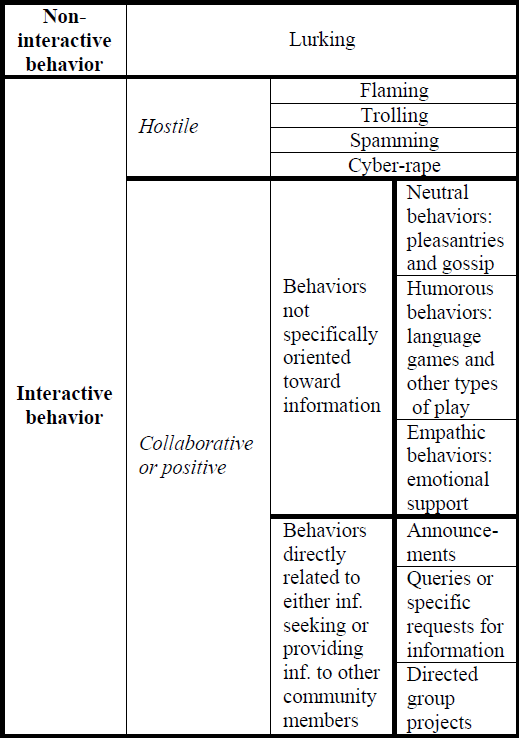
\includegraphics[width=0.45\textwidth]{../images/burnett.png}
\caption[Burnett's typology of online behaviour]{Burnett's typology of online behaviour (2000)}
\label{fig:burnett}
\end{figure}

\subsection{The changing face of \glsfmtshort{CMC}}

Between the mid 1990s and the mid 2000s, the nature of \gls{CMC}---and consequently, \gls{CMC} research---underwent a period of rapid change. As the result of a number of interwoven factors (the growing affordability of home computers; increasingly digital literacy; the development of early social network sites, etc.) the landscape of the Internet shifted from being primarily static and text\hyp{}based to dynamic, multimodal and participatory in nature \cite{herring_discourse_2011,lindholm_identity_2012}. The three currently most popular websites according to \emph{Alexa} in 2016 (\emph{Google}, \emph{YouTube} and \emph{Facebook}) exemplify this shift, in that each allows a great deal of user\hyp{}input and provides content in textual, audio and graphic modes. \textcite{herring_discourse_2011} reimagines the typology of familiar, adapted and new genres proposed by \textcite{crowston_reproduced_2000} to relate the dominant text types of `Web 2.0' to those that came before. Importantly, she notes that web genres can shift toward new\slash emergent as they mature, gaining features and responding to users' needs.

\subsubsection{Revisions of key claims in CMC research}

The profound nature of the shift to `Web 2.0' has meant that much early \gls{CMC} literature has now lost some of its relevance or explanatory power. Research into email messages is problematised by the fact that social media has overtaken email as the \gls{CMC} mode of choice for most digitally literate citizens \cite{thorne_computer-mediated_2008}, and by increasingly blurred boundaries between synchronous and asynchronous \glspl{mode}, such as email and instant messenger services. Similarly, the anonymity posited as critical to the discourse of early \gls{CMC}, while still possible, is no longer the norm: on social networking sites such as Facebook, \glslink{member}{users} communicate through personal accounts, disclosing their identities as they communicate and often even rendering the communication viewable to family and friends \cite{boyd_social_2007}. Furthermore, given that social networking sites are multimodal, and often contain a mixture of synchronous and asynchronous interactions, research informed by a characterisation of the Internet as fundamentally text\hyp{}based, or dealing exclusively with synchronous or asynchronous communication, is of limited usefulness for researchers of contemporary, often multimodal, \gls{CMC}.\endnote{For example, the myriad studies of communication on \emph{Usenet}---the text\hyp{}only Internet communication system in which many of the social elements of \gls{CMC} were first popularised---have been made largely redundant by the decommissioning of Usenet servers in 2010 \cite[e.g.][]{berge_computer-mediated_1995,eklundh_use_1994,jaffe_gender_1995}. That said, researchers have noted that despite greater bandwidth and the potential for multimodal interaction, in many respects, \gls{CMC} has remained surprisingly text\hyp{}based.}

In addition to the problem of reduced applicability, the findings of earlier research have since been challenged by research from the previous two decades \cite{herring_computer-mediated_2001,postmes_formation_2000}. As early as the mid 1990s, the characterisation of \gls{CMC} as impersonal, ineffective and hostile had come into question: \textcite{walther_computer-mediated_1996} argued that many early findings were caused by researchers' placing time restrictions on the observed \gls{CMC} interactions. If \gls{CMC} interactions are given unlimited time, Walther contends, they can achieve the same level of depth as face\hyp{}to\hyp{}face scenarios, both in terms of task\hyp{}completion and in the development of social relationships. In fact, Walther notes the potential for \emph{hyperpersonal} interaction in CMC: due to an optimised presentation of the self \cite[now often called \emph{self\hyp{}curation}; see][]{van_kleek_self_2015}, as well as idealisation of the Other, \gls{CMC} groups were found to be more polite and intimate than a face\hyp{}to\hyp{}face counterpart. Walther thus recognises two critical facts about interaction online: first, computer\hyp{}mediated interaction can be more candid than what could be observed in a comparable face\hyp{}to\hyp{}face setting; second, relationships develop in \gls{CMC} just as they do offline, necessitating longitudinal research. 

%From this perspective, aside from the slower pace of interactions, synchronous text\hyp{}based \gls{CMC} and face\hyp{}to\hyp{}face communication can be conceptualised as fundamentally similar in nature \cite{osullivan_reconceptualizing_2003,walther_interpersonal_1994,wu_is_2013}. The rapid increase in access to \gls{CMC} since this study 

The notion of a genderless and egalitarian Internet has faced similar scrutiny: \gls{CMC} research has shown that gender in anonymous, text\hyp{}only \gls{CMC} is often encoded by the \glslink{lexicogrammar}{lexicogrammatical} choices of the writer, as well as through the use of gendered discourse strategies such as assertiveness, politeness and aggression \cite{herring_gender_2000}. Likewise, education level is conveyed through vocabulary and complexity of message structure, and age through the discussion of interests and life experiences \cite{herring_computer-mediated_2001}. These findings echo the \glslink{SFL}{systemic-functional} notion that \emph{context is in text}, rather than around it, and can thus be reconstructed from linguistic analysis \cite[see Section \ref{sect:sfl}, as well as][]{eggins_introduction_2004}. Finally, research from the perspective of \gls{CDA} has questioned the notion of an egalitarian Internet at two separate levels. At the level of discourse, newer studies show that complex and rigid power structures exist online, even in low\hyp{}bandwidth \glspl{forum} and discussion lists \cite[e.g.][]{stommel_online_2010}. More broadly, contemporary theorists acknowledge that the landscape of \gls{CMC} has `inherit[ed] power asymmetries from the larger historical and economic context of the Internet', with a notable over-representation of English speaking, white males positioned as moderators, webmasters, and page creators \cite[p.~12]{herring_computer-mediated_2001}.

%Data and metadata are commodities: a main source of revenue for micro-blogging website Twitter is its \emph{Firehose}---an API that allows customers access to 500 million tweets per day. Researchers have attempted to mine tweets to detect natural disasters; to play the stockmarket; to aggregate content for entertainment websites. Each of these tasks requires the extraction of information from natural language.

\subsection{Contemporary CMC and its affordances for research}

%Though the Web is becoming more and more multimodal, methods for analysing human behaviour based on creation and consumption of multimodal content are only emerging. Multimodal content is very difficult to process automatically---typically, a great deal of manual effort is needed to transform multimodal content into data, and from data into insight. Plain text and metadata, however, are easier to transform into data, easier to annotate, and easier to search.

%todo: possible conflict between gruba and robyn re: future proofing ... i've deleted 'By 2016'
\gls{CMC} has now become become a central component of daily life, accounting for an ever\hyp{}increasing proportion of all human communication. Today, \gls{CMC} is used to contact those already close to us, rather than like\hyp{}minded strangers. Instead of well\hyp{}defined sessions of \gls{CMC} at a home computer, \gls{CMC} is now dispersed through work, travel and social occasions, and facilitated by an interconnected ecosystem of smartphones, tablets, laptops and desktop computers. Media convergence has led to new genres of communication, between journalists and readers, or companies and customers. The current Web therefore provides language examples that cannot be obtained through other means \cite{harvey_disclosures_2012}, or which have no antecedent in face\hyp{}to\hyp{}face discourse \cite{herring_discourse_2011}. As such, analysis of \gls{CMC} texts becomes necessary for investigation of many longstanding aims of linguistic research, including how language changes or evolves, how language is used to form and attend to social relationships \cite{canary_relationship_2015}, and\slash or how language is used to construe the human experience of the world.

\section{Healthcare and online communities}

% bit of a jump here ... 
Health discourse, in some form or another, is a large part of the landscape of contemporary \gls{CMC}---72 per cent of adult Internet users in the U.S. report having searched for health\hyp{}related content online \cite{fox_health_2013,fox_social_2014}. As mentioned in Chapter \ref{chap:intro}, talk about health covers a spectrum of registers \cite[in the systemic-functional sense\textemdash{}see][as well as Section \ref{sect:sfl}]{halliday_introduction_2004}. Ideationally, healthcare is a key topic online, with information about every conceivable symptom, illness and treatment strategy readily available through search engine results. Textually, health is represented in every popular \gls{mode} of \gls{CMC}, including wikis, blogs, online news, chatrooms, static information pages and mobile apps. Interpersonally, online health information targeting \glspl{consumer}%
\endnote{Interpersonally, not all health information online targets consumers---there are also sites with information for health professionals, academics, and so forth. These, however, are not relevant to the thesis.}
may be authored by governments, non\hyp{}profit organisations, health professionals, researchers, journalists, or, importantly, by healthcare consumers themselves. The latter of these---personal experiences with healthcare, authored by those living with health problems, and those who care for them, have significant public demand: a quarter of surveyed U.S. adults report specifically seeking out \glspl{consumer}' subjective accounts of their experiences with illnesses and journeys through healthcare systems \cite{fox_social_2014}.

Much consumer\hyp{}generated talk about health goes on inside dedicated online communities\textemdash{}that is, `mediated social spaces in the digital environment that allow groups to form and be sustained primarily through ongoing virtual communication processes' \cite[p.~986]{shen_effects_2013}. These communities most commonly exist within social networking sites (e.g. Facebook groups, Subreddits) or within bulletin board\slash \gls{forum} platforms\textemdash{}text-based \glspl{mode} of \gls{CMC} where registered \glslink{member}{users} can create and reply to \glspl{thread}. In academic literature and beyond, health\hyp{}oriented \glspl{forum} have been conceptualised as \glsxtrfullpl{OSG}\textemdash{}an online permutation of more traditional support networks for people living with health problems, or for those who care for them.

\glslink{forum}{Forum}\hyp{}based online communities and \glspl{OSG} have long been used as data sources for linguistic research due to their size, ubiquity and the ease with which they can be accessed: access to \glspl{forum} is round\hyp{}the\hyp{}clock and global; recording and transcription are unnecessary; and in many cases linguistic data is accompanied by rich, well\hyp{}structured demographic metadata \cite{leech_new_2006}. In general, empirical studies have shown that when contrasted with face\hyp{}to\hyp{}face equivalents, online communities have fewer barriers to entry, higher dropout rates and a comparatively high proportion of peripheral membership---that is, a greater rate of inexperienced or new members, compared to longstanding veterans \cite{sandaunet_challenge_2008,zhang_peripheral_2001}. That said, the efficacy of comparisons and contrasts between face\hyp{}to\hyp{}face and computer\hyp{}mediated communities has recently been questioned, as daily life becomes increasingly mediated by and merged with digital technologies \cite{wu_is_2013}. Indeed, a great number of users of \glspl{OSG} have never attended the offline antecedent of the \gls{mode}.

Linguists have paid attention to the central role played by language in online communities and \glspl{OSG}. It has long been argued by researchers that the limited semiotic resources available in many online environments (chiefly, a lack of physical co\hyp{}presence) makes language the most suitable resource for identity construction and role\hyp{}relationship negotiation \cite{thorne_computer-mediated_2008}. As \textcite[p.~303]{lam_language_2008} notes, `language practices are instrumental in creating the norms of behavior of particular online groups and how these norms function to provide sociability, support, information, and a sense of collective identity'. A similar perspective is provided by \textcite{postmes_formation_2000}, who argues that social identity issues have a stronger presence in \gls{CMC} environments, due to the de\hyp{}individuation that occurs in part due to reduced cues online. Because \glspl{OSG} facilitate intra\hyp{}consumer exchange, and because of the centrality of language to this task, the main thrust of linguistic online community and \gls{OSG} research has been toward language as an interpersonal, rather than an ideational resource---that is, toward the ways in which language is used to enact social relationships, rather than as a means of construing reality. Many studies have focussed on differences in communicative practices over the course of membership\textemdash{}most typically, on how newcomers position themselves as legitimate prospective members whose contributions deserve replies, and how longer\hyp{}term members represent their expertise and construct\slash reinforce normative community values. In the sections that follow, I review key \glspl{theme} in linguistic accounts of interpersonal meaning\hyp{}making in online communities, with preference given to \gls{forum}\hyp{}based or health\hyp{}oriented communities where available.

%In health contexts, the centrality language provides an attractive possibility for research into \gls{consumercentred} care, which similarity shares an interest in interpersonal, rather than ideational meaning\hyp{}making. % includes section on online community

%\input{chapters/cmd.tex}

% NEW MEMBERS
    % legitimacy

% VETERAN MEMBERS
    % van leeuwen
    % legitimacy
    % the lay expert

% LONGITUDINAL CHANGE
    % socialisation

% SHORTCOMINGS
    % qualitative
    % non-systemic

%todo: add %\textcite{pfeil_social_2011} show how core community members are more likely to adopt supporting
% Though we can easily infer longitudinal change in members' roles, the authors do not show this process occurring.


\subsection{New members, first contributions and legitimacy} \label{sect:newmembers}

People can sign up and begin contributing to most \glspl{OSG} at any time. A common practice is for new \glslink{member}{users} to create a new \gls{thread}, which serves as a self\hyp{}introduction, which outlines the user's motivation for having joined. Because drop\hyp{}out rates are high, such `first \gls{post} \glspl{thread}' are a constant feature in the landscape of many popular \glspl{forum}, and have thus received attention during studies of \glspl{OSG}.

There are broad interpersonal similarities between first contributions within many \glspl{OSG}. Generally speaking, new users attempt to carve out a social position from which it is possible to elicit certain kinds of language from others\textemdash{}that is, to increase the perlocutionary force of one's own utterances \cite{austin_how_1975,roberts_communicative_1996}. Most commonly, new \glslink{member}{users} want to be given information and social support after having requested it. This has been referred to as a position of \emph{legitimacy}, arrived at through an ongoing process of \emph{legimitation} through semiotic exchange \cite{davies_communities_2005,smithson_developing_2012,van_leeuwen_legitimation_2007}. In comparison to offline support groups, where physical co\hyp{}presence and extralinguistic communication can serve legitimating functions, new contributors to \glspl{OSG} instead exchange meaning and communicate legitimacy almost exclusively through the linguistic content of their \glspl{post} \cite{galegher_legitimacy_1998}. What kinds of language choices manoeuvre the \glslink{member}{user} into the legitimate position may vary, with individual community cultures shaping what messages contain, how messages are structured, and the kinds of replies they receive \cite{gallagher_what_2015}.

\subsubsection{Legitimation strategies in newcomer talk}

Because texts are structured in order to make things happen, and because one of the functions of first \glspl{post} is to legitimate the self, it is possible to look within the structure of these texts to see how legitimation is realised at the strata of \gls{lexicogrammar} and \glspl{discourse-semantic}. Commonly, first \glspl{post} are designed to demonstrate the fulfillment of explicit, implicit or perceived community membership criteria. \textcite{varga2014grieving} qualitatively analysed more than 100 first \glspl{post} to an \gls{OSG} for grief, with the purpose of unpacking the ways in which new users socially construct grief in a way that elicits useful responses. Three main strategies were identified: presentation of an atypical story, of an uncontrollable emotional state, and through \emph{troubles telling}\textemdash{}\glspl{post} in which the new \glslink{member}{user} explains a problem but does not explicitly request advice. 
%The analysis of pairs of request and response is indeed the best way to obtain a useful sketch of the ways in which advice is dispensed, and the underlying motivations for each choice. This kind of approach also poses problems for \gls{CL} methods, however, as few \gls{corpus} are annotated in such a way as to link the initialisation and response components of the text.

Similarly, \textcite{smithson_membership_2011} describes the legitimating function of first \glspl{post} to an \gls{OSG} for self\hyp{}harm: new \glspl{member} were observed setting out their credentials for group membership, giving narrative medical histories, utilising medical jargon and making reference to other related communities in which they have participated. This finding is echoed by \textcite[p.~5]{varga2014grieving}, who find that `story formulations often serve particular functions in discourse, such as displaying affiliation with a group and establishing eligibility for group membership'.

\textcite[p.~173]{horne_doing_2009} use discursive psychology as an underlying theoretical framework to analyse the structural and functional components of first \glspl{post} to a suicide \gls{OSG}. They explore the difficulty faced by \glspl{member} who present as suicidal, but whose continued presence in the \gls{forum} casts doubt upon the legitimacy of their claim. Three major types of messages are identified: \emph{life narratives}, in which a medical history is presented without a specific addressee; \emph{immediate threats}, which are typically short, containing present and future tense; and \emph{requests}, which involved requests for advice, and the use of mainstream medical terminology. The latter category received the fewest replies. The authors hypothesise that this is due to a lack of urgency within the lexicogrammatical choices of \emph{request} \glspl{post}, leading to an impression that the new \gls{member} is `inauthentically suicidal' \parencite*[p.~180]{horne_doing_2009}. At the same time, explicit requests for advice construct potential responders as equally inauthentic, as it casts them as using the \gls{OSG} for purposes other than support seeking. 

\textcite{stommel_use_2011} adopt \gls{CA} as a way of showing how new \glslink{member}{users} in an eating disorder \gls{forum} engage in self\hyp{}legitimation by construing themselves as formally diagnosed with a disorder. While having a diagnosis is not an explicit community rule, the authors argue that it nonetheless functions as an `entry ticket' for continued participation within the group \parencite*[p.~6]{stommel_use_2011}. Though this is an interesting suggestion, so far lacking is a detailed investigation of the syntagmatic behaviour of the diagnosis event as it is construed in \gls{OSG} texts: if the process of diagnosis functions as an `entry ticket', we might expect that it is construed metaphorically as a participant, so that it can be classified and possessed.

\textcite{stommel_use_2011} also show how newcomers often express reluctance to participate and insecurity concerning the content of their first \gls{post}. These hesitations are marked in  the lexicogrammar, by modal auxiliaries and adjuncts, and by ellipsis, which may be marked graphologically with ellipses \parencite*[e.g. \emph{I'm still a bit unsure about what I should write \dots---}][p.~4]{stommel_use_2011}. The authors argue that marking hesitation allows the new user to appear equitable and well\hyp{}prepared. It also indicates a level of respect for the opinions of the rest of the community, communicating an intent to take replies seriously. 

\subsubsection{Structure of first posts} \label{sect:post-structure}

Some authors have commented on the overall structure of first posts. \textcite{varga2014grieving}, for example, note that new threads posted to the \gls{OSG} for grief often conform to common structure:

\begin{quote}\small\singlespacing
We found that newcomers opened their initial \glspl{post} with stories that began at the event of loss and then moved to establish the background of their relationship with the deceased. Emphasizing the unusual circumstances of their loss and the depth of their connection with the deceased provided an account for their grief. Newcomers continued their accounts through descriptions of their uncontrollable emotional and physical symptoms, which worked to display affiliation with \glspl{member} of the group and to make the case for their legitimate entry \parencite*[p.~5]{varga2014grieving}. 
\end{quote}
%
%\noindent The authors point out, however, that their qualitative approach limits the generalisability of the study, noting that further research is necessary to confirm their exploratory results.
%
Similar structural components---the narration of a personal (medical) history, and its lead\hyp{}up to a current problem---have been identified in other analyses of \glspl{OSG}. \textcite[p.~4]{weber_missed_2011} analyses the role of dispute and conflict in the socialisation process of new \glspl{member} of an online sexual abuse support group. She provides a basic account of the generic structure of newcomers' \glspl{post}:

\begin{quote}\small\singlespacing
Contents typically found in newcomers' messages include: a greeting; a description of the person's contact with the group thus far; a reference to sexual abuse experiences or related problems; and a request.
\end{quote}
%
Using terminology from \textcite{goffman_presentation_1959} and \textcite{brown_politeness:_1987}, Weber makes a case that this structure represents an \emph{entrance frame}: during each component of the frame, devices such as humour, insecurity, and unease can be used to both perform identity and to set up an exchange with a lessened potential for loss of face or redress. 

%todo: clarify typographical conventions
Using the framework for narrative stage analysis outlined by \textcite{labov_narrative_1997}, \textcite{kouper_pragmatics_2010} provides an account of the structure of initial \glspl{post} to a \emph{LiveJournal} community. She notes that messages contain sequences of \sctext{ORIENTATION}, \sctext{PROBLEM DISCLOSURE}, \sctext{REQUESTS} (for advice and for information; of varying degrees of explicitness) and \sctext{JUSTIFICATION} for posting. Because there was no hard limit on the size of a contribution (as is typical of \glspl{OSG}), all stages aside from the \sctext{ORIENTATION} can occur multiple times in a single text. No component was found to be obligatory in every message.

%Because it is possible to remain a lurker in many \glspl{OSG}, the act of self-introduction itself, irrespective of its linguistic content, is an act that demonstrates desire for membership.

\subsubsection{Limitations in current understanding of newcomer talk} \label{sect:limit-newcomer}

% not really important ...
A potential methodological issue in the work of \textcite{horne_doing_2009} \citeNP[as well as others, e.g.][]{stommel_online_2010} is that the authors treat the presence or absence of replies as indicators of a \gls{post}'s `success'. While this may be a sensible or convenient assumption when doing larger, quantitative\hyp{}based studies of number of replies, it is perhaps less reliable in small\hyp{}scale qualitative research: there is no explicit evidence concerning whether or not replies would have been posted if the first \gls{post} were written differently. Moreover, when using publicly available \gls{forum} data, there is no reliable way to tell that \glspl{post} were even seen by those who would be likely to reply. Another key factor in whether or not replies are received is the user's profile: \textcite{feng_is_2016} find that \gls{OSG} participants with recoverable first names and portraits as avatars receive friendlier, more personalised replies than do more highly anonymised users. In general, however, this factor has not been taken into account in related literature.

%\textemdash{}a phenomenon known as \emph{lurking} common to many \glspl{mode} of \gls{CMC}
A second key issue in the study of new \glspl{member} and initial contributions is the potential for a user's first experience with the community and his\slash her first contribution to it to be conflated. Though first \glspl{post} represent the first time a user actively engages in a discussion, he\slash she may not in fact be new to the community: users may have signed up or read through \glspl{post} for any length of time before choosing to post. Some first contributions, therefore, are made by people who have just discovered the community and are unaware of its normative communicative practices, while others are made by \glspl{member} who are already intimately familiar with the community's discursive norms \cite{dennen_pedagogical_2008,han_social_2012,preece_top_2004,smithson_membership_2011}. \textcite{weber_missed_2011}, for example, shows that long\hyp{}time lurkers often draw upon the normative genre and register appropriately when they first decide to author a \gls{post}. Such \glslink{member}{users}, she finds, often flag in their \glspl{post} the fact that they have lurked for extended periods before posting, in order to account for their level of familiarity with the lexicogrammatical, discursive or ideological orientation of the group. The phenomenon of lurking therefore poses a specific challenge to particular theoretical conceptualisations of group dynamics. Socialisation theory, for example, in stressing the notion of learning through active participation, may become an unsuitable model for interpreting communities where a great deal of learning may take place non\hyp{}interactively.
% Reasons for this are potentially contradictory: users may flag their newcomer status in order to provide a reason for their breaking explicit or implicit community rules; alternatively, user
%for approaches to online community\slash\gls{OSG} membership informed by socialisation theory, for example ow), which stresses the process of learning through active participation.

A final limitation in existing work on first posts to \glspl{OSG} is the dominance of bottom\hyp{}up, \gls{CA}\hyp{}informed approaches. While \gls{CA} is certainly suitable for exploratory, qualitative and discourse\hyp{}analytic work, it is not intended to uncover generalisable relationships between linguistic system and language instance. For this reason, \gls{CA} is not typically used in large\hyp{}scale quantitative investigations, which access discourse through automatic location of lexicogrammatical phenomena, and manual abstraction of the meaning of these phenomena via a grammar. \gls{CA}, therefore, while useful as a way of identifying legitimation strategies, has not provided an explicit description of how legitimation may be realised in words and wordings. This limits the ability to perform automated feature discovery or frequency counting, as well as the ability to uncover register differences based on fluctuations in frequencies of lexicogrammatical phenomena.

\subsection{Veteran membership and legitimacy} \label{sect:vetmemb}

A smaller proportion of \gls{OSG} legitimacy research has concerned the language use of veteran members, especially as replies to initial contributions \cite{paulus_`please_2015}. As noted in Section \ref{sect:intro-lang-in-osg}, these studies address a hypothesised concern from earlier \gls{CMC} theory that \glspl{member} may take advantage of the lack of social cues in the online community and linguistically convey a level of expertise or legitimacy that is at odds with their actual level of health literacy or knowledge \cite{varga2014grieving}. Evidence regarding the existence and ramifications of this phenomenon is conflicting, however \cite{sillence_giving_2013}. \textcite{hoch_information_1999}, for example, found that six per cent of all advice provided in an epilepsy \gls{forum} was objectively wrong. Similarly, \textcite{hoffman-goetz_clinical_2009} concluded that nine per cent of information in a diabetes community deviated from clinicians' guidelines. On the other hand, Sillence's study of a breast cancer \gls{forum} found that `only a very small amount of messages observed in the present study reflected a lay belief or misbelief in [patient-controlled analgesia] treatment' \parencite*[p.~8]{sillence_communicating_2012}. \textcite{smithson_problem_2011} reported that in contrast with researchers' expectations, replies to new \glspl{member} of a self\hyp{}harm \gls{forum} were almost always found to be surprisingly mundane and conservative in nature, with `go and visit the GP' being by far the most common advice dispensed. Research has also yet to show a conclusive link between incorrect or poor quality information online and negative treatment outcomes. As \citeauthor{wang_stay_2012} explains:

\begin{quote}\small\singlespacing
It is highly likely that the effectiveness of such groups depends on the communications that \glspl{member} exchange with one another, but surprisingly little systematic research has been devoted to specifying how the quality and quantity of such communications affect groups' outcomes and members' health\hyp{}related outcomes \parencite*[p.~1]{wang_stay_2012}.
\end{quote}

In general, analyses of \glspl{OSG} have shown that long\hyp{}term \gls{forum} \glspl{member}' language use differs from that of newcomers in a number of respects. Veterans are more likely to welcome newcomers, speak on behalf of the \gls{forum} and its other members, dispense advice and instructions, and\slash or act as gatekeepers by ratifying or rejecting membership bids \cite{paulus_`please_2015,pederson_supporting_2010,weber_missed_2011}. As such, these \glspl{member} are usually understood as being in a position of power, or higher social standing, than the newcomers they address.

Inspired in part by \gls{SFL} theory, \textcite[p.~92]{van_leeuwen_legitimation_2007} proposes four major discursive strategies for legitimation used by those in positions of power: \emph{authorisation} (reference to `persons in whom institutional authority of some kind is vested', potentially including both the speaker him\slash herself and\slash or those with whom he\slash she agrees), \emph{moral evaluation} (reference to venerated social values), \emph{rationalisation} (references to hegemonic social action) and \emph{mythopoesis} (narratives casting legitimate action and those who perform them in a favourable light). Informed by \gls{SFL} and \gls{CDA}, \textcite[p.~782]{reyes_strategies_2011} augments Van Leeuwen's framework for the purposes of accounting more specifically for the ways in which social actors construct legitimate action through the use of emotion, the description of hypothetical future outcomes, and through displays of altruism. %Realisations of these strategies in grammar are diverse. % The appraisal framework is useful as a means of analysing emotional language;

The kinds of legitimation strategies described by \textcite{van_leeuwen_legitimation_2007} and \textcite{reyes_strategies_2011} have been empirically observed in the language of those who respond to newcomers' \glspl{post}. Particularly relevant is legitimation via reference to personal authority. First, a number of studies have highlighted the framing of health professionals as authorities. \textcite{smithson_problem_2011} and \textcite{vayreda_social_2009} have found that advice dispensed by veterans often aligns with a biomedical ideology, in which the health professional is the definitive source of knowledge, as well as the agent behind critical points in the consumer journey such as diagnosis. Second is the framing of the self and other veteran \glspl{member} as authoritative. Van Leeuwen distinguishes between three different subtypes of authoritative legitimation: \sctext{personal} (in which the authority figure and the target are in a culturally recognised hierarchical relationship, such as student\slash teacher or child\slash parent), \sctext{expert} (where the authority figure has relevant experience that is lacking for the target) and \sctext{role model} authority, where actions are justified on the basis that they are also performed by people that the target may respect or admire). Grammatically, authoritative legitimacy often involves verbal and mental processes with the authority positioned as Sayer\slash Senser. The personal subtype is likely to also involve high\hyp{}obligation modality (\emph{she said that we should go}\textemdash{}see Section \ref{sect:sfl} for an elaboration of the \gls{SFG}). Veteran \gls{OSG} \glspl{member} have been shown to variously fulfill each of the three subtypes. They may explicitly moderate problematic content or ban \glslink{member}{users} who break rules \cite{weber_missed_2011}. They may provide expertise by providing health information in an objective, impersonal Tenor, as a set of facts \cite{kaufman2016producing}. Alternatively, they may self\hyp{}present as role models, providing health information and advice alongside personal narratives from their ongoing consumer journey \cite{koteyko2015performing}.

%Appeals to tradition and conformity
%The notion of legitimacy can be applied here too; that said, the strategies for becoming legitimate are generally different, as are the desired perlocutionary effects that come from the legi
%Veteran \glspl{member} may want to have a say in the overall direction of the community; they want their demands on others (advice giving, or requests for follow-up information) to be heeded.
%As \textcite{eggins_analysing_2004} point out, understanding the ways a text is responded to is key to understanding its original purpose. \textcite{harrison2009politeness} note that phenomena such as politeness and advice are bound to context; interpretation of the ways people react to others is critical to proper understanding of intentionality.

\textcite{kaufman2016producing} use a combination of \gls{CA} and discursive psychology to analyse replies in an \gls{OSG} for depression and their usefulness as social support devices. They note that responders to first \glspl{post} communicate empathy through a two\hyp{}part structure of explicitly claiming to feel empathy (e.g. \emph{I feel the same way}) followed by a demonstration of a shared trouble, and, potentially, a construal of the speaker as role model:

\begin{quote}\small\singlespacing
I went through the same things that you are going through right now about 2 years ago. I PROMISE you that things will get better. The way that got me out of being depressed is by taking out my anger and sadness on making music or writing stuff down on some paper \parencite*[p.~8]{kaufman2016producing} 
\end{quote}
%
Unlike most \glspl{OSG} research, the authors problematise the distinction between information and support provision: in cases such as depression, psychoeducation can relieve symptoms by normalising the experiences of the addressee. As such, even objectively presented health information functions as a gesture of social support. Likewise, the authors point out the reciprocal nature of offers of empathy within the depression community. Those who respond to new \glspl{thread} (most typically, veteran \glspl{member}) are also benefiting from the exchange, in being given a platform and space with which to engage in a kind of talk therapy. As such, provision of support by veteran \glspl{member} may simultaneously affect the second person (the addressee), the third person (other community \glspl{member} and readers) and the first person (the self). More directly, \textcite{pudlinski_giving_1998} has shown that sharing related stories may in fact elicit direct social support from the addressee---in this way, part of the motivation for the responder is to receive the same manner of support that he\slash she is providing in the response.

%They note that lacking in the existing literature have been analyses that connect features of \gls{OSG} texts to the efficacy of the communities as sites of social support.

\subsubsection{Advice} \label{sect:advice}

Either explicitly or implicitly, studies of replies and\slash or veteran \gls{member} behaviour in \glspl{OSG} have often centred on the notion of \emph{advice}. Defined here as `opinions or counsel given by people who perceive themselves as knowledgeable, and\slash or who the advice seeker may think are credible, trustworthy and reliable' \cite[a definition taken from][p.~519]{decapua_strategies_1993}, advice is interesting due to its inherent ties to legitimacy, and due to its multifunctionality: advice has both interpersonal purposes (to cause the addressee to do something; to negotiate power dynamics) and experiential purposes (to construe facts and\slash or ideal behaviour) \cite{heritage_dilemmas_1992}. Peer\hyp{}to\hyp{}peer advice is also important for clinical research, given its potential influence over \glslink{member}{users}' healthcare decision making practices \cite{jones_health_2013,sillence_giving_2013}.

Linguistic perspectives on advice provision in English have been provided by \textcite{hudson1990discourse}, \textcite{decapua_`if_1995} and \textcite{decapua_strategies_1993}. Generally, the focus of these accounts has been on the directness of advice, whether or not it was solicited, and the influence of these factors on how it is received. Common is the recognition that advice is potentially face\hyp{}threatening, and as such, its realisations are diffuse within the grammar. Advice is often accompanied by hedging strategies, including incongruent mood choices, modalisation, or politeness markers: `even solicited advice\hyp{}givers can resort to a variety of stylistic and linguistic means to protect themselves from accusations of unfairly taking on the role of ratified experts' \cite[p.~126]{decapua_`if_1995}. A given instance of advice may therefore have agnate realisations as an imperative (\emph{Go and make an appointment}), a declarative (\emph{You should make an appointment}) or an interrogative (\emph{Could you make an appointment?}).

\textcite{kouper_pragmatics_2010} investigates an online motherhood community hosted by \emph{LiveJournal}, focussing on both realised forms of advice, and the structure of the \glslink{post}{text} to which the advice giver is responding (see Section \ref{sect:newmembers} for studies of first \glspl{post}). Occurrences of advice in a one\hyp{}month sample of contributions were coded according to four categories: 

\begin{enumerate}\small
\item Direct advice (Any comment that included imperatives or the modal verb \emph{should})
\item Hedged advice (Any comment that contained explicit hedges, hedging devices, or softeners of various types)
\item Indirect advice (Any comment that had no explicit or hedged advice, but had enough information to act on it)
\item Description of personal experience (Any comment that had no explicit, hedged advice, or indirect advice, but had an account of how the person dealt with the situation an advice seeker had described) \cite[adapted from][p.~7]{kouper_pragmatics_2010}
\end{enumerate}
%
The categories are primarily designed to distinguish directness of advice, with grammatical distinctions naturally playing an important, but secondary role. Notably, imperative and \emph{should}-modalised declarative are understood as equally direct---a classification at odds with the \gls{SFG}, where \sctext{Modality} is a more delicate grammatical component than Mood Type. Also of interest to the case study of this thesis and its associated methods is the most indirect kind of advice, which has no explicit grammatical criteria. An example is provided:

\begin{quote}\singlespacing\small
beautiful becca :) i gave wesley a bath every 2-3 days. but now he is 10 weeks old and i bathe him every night because he loves his bath time so much  \textcite[p.~13]{kouper_pragmatics_2010}.
\end{quote}
%
Naturally, such indirect realisations are a complicating factor for \gls{CL} approaches to advice, which may struggle to automatically locate instances that are not indexed by any one particular \glslink{lexicogrammar}{lexicogrammatical} feature. This is discussed in more detail in Chapter \ref{chap:discuss-bp}.

Advice research has also highlighted the fact that strategies for advice provision are affected by the roles and relationships of interactants. \textcite{decapua_`if_1995} shows how the use of unhedged imperatives, for example, is more likely in contexts where the difference in status between advice giver and receiver is obvious, explicit and\slash or institutionally prescribed. Interactions between speakers of similar social standing are more likely to feature more hedging, including modalisation, and declarative Mood. In such contexts, \citeauthor{decapua_`if_1995} note, advice giving and requesting can foster interpersonal closeness through \emph{(i.)} the determination and exchange of shared values, \emph{(ii.)} flattery, by a positioning of the advice giver as knowledgeable, and \emph{(iii.)} potentially intimate personal revelations.

% LOCHER
Advice online has been investigated extensively by Locher \parencite*{locher2006advice,locher_health_2010}, focussing mostly on an online advice column called \emph{Lucy Answers}. Locher's interest is primarily in what she calls \emph{interpersonal pragmatics} or \emph{relational work}---what may in \gls{SFL} be understood as \emph{interpersonal \glspl{discourse-semantic} or meaning}. Her approach relies on manual annotation of various syntactic and semantic features of the questions asked to the columnist and her replies. 

For her analysis of relational work, Locher codes the columnist's responses with seven relatively broad semantic categories: \emph{bonding}, \emph{boosting}, \emph{hedging}, \emph{praising}, \emph{emphasizing}, \emph{criticizing}, \emph{humor}. Categories may contain subcategories (to reflect, for example, the hedging function of humour), and multiple categories may be applied to a part of a text. She finds that hedging is a very common strategy, related to the overall genre of the column. Lucy the advice giver fosters a sympathetic relationship with readers and contributors, rather than a hierarchical one. Hedging lessens the difference in social status that may stifle the candid kinds of language use that the column's readers enjoy. These categories differ in the extent to which they can be mapped to particular features of the \gls{lexicogrammar}: Locher's examples of \emph{hedging} are typically examples of modulation (\emph{maybe}) or modulation via grammatical metaphor (\emph{It is important that you ...}); \emph{humor}, however, mostly relies on the judgement of the analyst, the recognition of wordplay, and the like. Because these kinds of features differ in the extent to which they are indexed in grammar, they also differ in the extent to which they can be identified automatically using computational tools and methods.

\textcite{locher2006advice} also employs counting of lexicogrammatical features, which can more reliably be counted using methods from \gls{CL}. When analysing the ways in which Lucy dispenses advice, Locher codes texts for Mood Type, finding that declaratives, often modalised, are the most common (52\%), followed by imperatives (36\%), and interrogatives (11\%). These results are contrasted with other studies of advice in contexts such as face\hyp{}to\hyp{}face or radio, which more commonly feature imperative realisations. She argues that the orientation of the advice column `toward facilitating decision processes' (p.~132) is responsible. In situations where the potential for losing face is less critical than effective prescription of a course of future behaviour, direct forms are likely to be preferred.

%in high-stakes, professional--consumer medical contexts, for example, 

There are two major limitations in Locher's work for investigating advice in online health communities. First are apparent inconsistencies and contradictions in Locher's lexicogrammatical analyses. In the context of advice, Locher analyses declarative as being `suggestions', interrogatives as `inviting future action', compared with imperatives, which issue `directives'. Because some examples of declaratives appear to be directives (\emph{You need to go ...}), however, Locher reclassifies declarative $+$ \emph{need}\slash \emph{should} as imperatives, arguing that `in written sources such as advice columns, a preference for imperatives and imperatives with \emph{should} or \emph{need} was found' (p.~39), despite the fact that \emph{should} cannot grammatically modalise an imperative clause. This is a conflation of grammatical Mood Type (imperative) and the speech function it typically realises (a command). A related issue is the conceptualisation of \emph{hedging} as a phenomenon distinct from Mood Type choice. Advice such as \emph{See your doctor}, when realised as an interrogative (\emph{Would you consider seeing a doctor}) is perhaps better understood as a hedged form of the congruent command---especially in the advice column genre, where the question cannot possibly receive an answer.

%`When declarative sentences are used to realize advice, they can best be described as suggestions. (p.~192)

The second issue is that there are a number of critical medium and situational factors that differentiate online (forum\hyp{}based) communities from the \emph{Lucy Answers} online advice column. These differences can be understood with reference to the register dimensions of Tenor, Mode and Field from systemic linguistics \cite{halliday_language_1989}. In terms of Tenor, the advice column is an interaction between a pseudonymous advice seeker living with a health problem and a named, institutionally prescribed expert, who is responsible for selecting questions for publication and response. This power imbalance is likely to manifest in the ways in which advice provision is distributed amongst \sctext{Mood} and \sctext{Modality} systems: following \textcite{decapua_`if_1995}, we could expect that imperative provision of advice, for example, would be more common within the \emph{Lucy Answers} dataset than in most online \glspl{forum}, where contributors share a common identity as sufferers of a condition, differentiated hierarchically only by membership length and number of \glspl{post}, rather than by codified institutional roles. In terms of Mode, interactions within the advice column are limited to an initial question and a single response---in many respects, a reconfiguration of the advice column genre found in newspapers and magazines \cite[see][]{herring_discourse_2011}. As such, there is no longitudinal development and negotiation of role\hyp{}relationships between the two interactants, nor any way to track the health journey of the advice seekers after their contribution has been made. Compared with Tenor and Mode, the dimension of Field remains more or less consistent, however, with both \emph{Lucy Answers} and online health \glspl{forum} broaching a broad array of topics related to not just health, but work and social relationships as well. Though \emph{Lucy Answers} is unlike most health \glspl{forum} in not being dedicated to a single health concern, this is likely to affect only the ideational meaning embedded in advice (i.e. the specific health problem and remedial action construed), and not the ways in which advice is interactively exchanged.

Related to Locher's work is that of \textcite{harrison2009politeness}, who investigate the linguistic negotiation of role\hyp{}relationships in an online community for arthritis. They categorise 255 advice moves by \sctext{Mood Type} using the same criteria as \textcite{locher2006advice}. Their findings are similar, with declaratives the most common (64\%), followed by imperatives (21\%) and interrogatives (15\%). They argue that this range of possible realisations is linked to the multifunctionality of the act: advice provides suggestions for future action while also reinforcing the veteran's claim to authority, and thus maintaining the hierarchical relationship between newcomer and veterans:

\begin{quote}\small\singlespacing
[Instances of advice] embody suggestions, while at the same time evidencing the writer's authority to make these suggestions: the narrative demonstrates the writer's experience of the recipient's problem, and the writer's chosen way of addressing the problem. Thus, through their narratives, the advice givers reflect on and give structure to their own experience, constructing their identities as expert patients \cite[p.~107]{harrison2009politeness}.
\end{quote}
%
While this study addresses the aforementioned concerns regarding the generalisability of Locher's work, and while it acknowledges the concurrent unfolding of interpersonal and ideational meanings in language, it nonetheless still provides only a general impression of the \sctext{Mood} and \sctext{Modality} probabilities of advice in online health \glspl{forum}: as with \textcite{locher2006advice}, \citeauthor{harrison2009politeness} do not provide a longitudinal account of interpersonal meaning\hyp{}making, nor an empirical account of the relationship between interpersonal status and lexicogrammatical choices.

Particularly relevant to this thesis is the study of a \gls{bipolar} \gls{forum} undertaken by \citeauthor{vayreda_social_2009}, which uses \gls{CA} to explore `an apparent contradiction between a new user's first post and \gls{forum} members' replies with ostensibly unsolicited advice' \parencite*[p.~931]{vayreda_social_2009}. It was found that new forum \glslink{member}{users} rarely explicitly asked for advice, but were provided with it regardless. The authors contend that advice was thus unsolicited, but complementary nonetheless: new \glslink{member}{users} made a `low bid' by only vague specification of the kinds of replies they sought; established \glslink{member}{users} took this opportunity to direct the user to shift toward group norms \parencite*[p.~940]{vayreda_social_2009}. This contrasts with \citeauthor{kouper_pragmatics_2010}'s finding that most advice was in fact solicited by the user who began the \gls{thread}. This contradiction is perhaps the result of the fact that \citeauthor{vayreda_social_2009} take a very narrow view of what exactly constitutes a request for advice, discounting formulations in which requests may be incongruently realised, as in the following:

\begin{quote}\small\singlespacing
`It'd be great if someone could share this first stage of acceptance with me, or tell me how they got through it.' \parencite*[p.~11]{vayreda_social_2009}
\end{quote} 
%
\noindent Here, though the new \glslink{member}{user} chooses a conditional declarative rather than a modalised interrogative as a means of realising a request, given that requesting advice involves deference and a potential loss of face \cite{brown_politeness:_1987}, such hedging does not seem inappropriate. Aware of the fact that expert \glspl{member} are fluent in the community's discursive norms, a new member could perhaps expect that such heavily modalised constructions could be unpacked and decoded as requests for advice. As \textcite{goldsmith2000soliciting} points out, while overt requests for advice open up a context in which advice can be provided without threatening face, general solicitation of opinions on a topic are often understood by the addressee as permission to advise. In a hierarchical community of newcomers and experts, this is especially likely, as the new \glslink{member}{user} understands that the veteran has personal experience with the nature of the problem. As \textcite{eggins_analysing_2004} remind us, rather than relying on linguistic intuition alone, the best way to disinter the intentionality of an utterance is often to analyse the utterances that follow. Given that such responses are apparently treated as advice by those who respond, this may suggest an underlying shortcoming in Vayreda and Antaki's classificatory scheme.

\subsubsection{The lay-expert\slash proto-professional}

In medical contexts, a well\hyp{}noted strategy for legitimation is the invocation of a \emph{lay\hyp{}expert} or \emph{proto\hyp{}professional} register, which is realised at both \glslink{lexicogrammar}{lexicogrammatical} and \gls{discourse-semantic} levels. Lexically, for example, such a register may involve the use or appropriation of medical jargon in lieu of lay terms \cite{harvey_disclosures_2012,sullivan_gendered_2003}; discursively, the lay\hyp{}expert has been shown to foreground personal experience and display emotional affect when construing medical fields \cite{wilson_expert_2007}. This conceptualisation, of a social role and associated linguistic repertoire that lies between novice and expert, is one useful lens through which we can understand language features of long\hyp{}term \gls{OSG} members.

\textcite{thompson_credibility_2012} examine the discursive features of lay expertise through interviews with members of \emph{patient and public involvement panels}\textemdash{}laypeople consulted by medical institutions in the U.K. in an attempt to involve the public in the medical research process. They noted that those in lay\hyp{}expert positions may champion their lack of formal medical training or employment, arguing that it affords a unique point of view that is uncorrupted by financial or socio\hyp{}political factors. Simultaneously, a high degree of deference to the opinions of health professionals was also observed: interviewed participants `not only supported the dominant techno\hyp{}scientific discourse around research, but also seemed to defer readily to it in place of their own experiential expertise' \parencite*[p.~609]{thompson_credibility_2012}. That said, these findings may be strongly influenced by the social context in which the interviews took place: as the participants of the study were afforded privileges and treated as having `honorary' roles by health professionals, their construction of both their unique perspective and health professionals' ultimate superiority may be influenced by the desire to maintain their current position and role. Indeed, studies of \glspl{OSG} where normative community values oppose those of mainstream Western medicine have noted that formal healthcare institutions, their participants and processes (e.g. hospitals, health professionals and diagnosis) are often cast in a negative light and treated sceptically by community members \cite{mulveen_interpretative_2006}. One of the advantages of \glspl{OSG} as sources of data, therefore, is access to the lay\hyp{}expert register uncorrupted by the presence and potential influence of healthcare professionals.

%Related is the already\hyp{}noted finding in \textcite{horne_doing_2009} that \gls{OSG} \glspl{post} aligned with mainstream opinion and featuring information about doctors' diagnoses were ignored by other \glspl{member}.

%In a \gls{CMC} context, \textcite{paulus_`please_2015} refer to `second\hyp{}stories', where veteran responses to newcomers' introductory narratives involve telling similar or related narratives from the journey of the veteran. These tales serve to normalise the new \glslink{member}{user's} problem and promote solidarity. Simultaneously, such stories have legitimating functions: they establish lay expertise

%Veteran \glspl{member} also speak on behalf of the community, by welcoming, or by explaining the purpose and orientation of the community:

%Veteran users perform legitimation through rationalisation, construing new users' actions and feelings as in line with the hegemonic social values of the board. \textcite{paulus_`please_2015} give the example of 

\textcite{koteyko2015performing} operationalise the notion of the lay\hyp{}expert in an online context, using ethnography and text analysis to qualitatively examine the ways in which Facebook users construct a representation of the self as a lay\hyp{}expert in communication about diabetes. Noting that social networking sites have received less attention within online health discourse literature than \gls{forum}\hyp{}based communities, they argue that such sites provide new, under\hyp{}researched channels through which semiotic health resources can be exchanged. The convergence of a number of (monomodal and multimodal) types of \gls{CMC} within Facebook's infrastructure (e.g. link sharing, microblogging, chat, photo albums, etc.), for example, give rise to a novel practice where users publicly share links to medical literature, accompanied by a `translation' or summary of its significance into simpler English for a lay audience.\endnote{The phenomenon of translating medical texts for new audiences, though possible in text\hyp{}based \glspl{forum}, is apparently very uncommon. No literature was found that discusses it; nor was it seen in the case study.} Lay expertise, therefore, is not simply communicated and constructed through talk, but through online activity more generally, with posting, replying, and `liking' others' content each contributing to the construction of identity. These kinds of practices, of course, are difficult to analyse through automated corpus linguistic techniques, which tend to strip away multimodal features of texts, and which may struggle to differentiate between individual voices in group discussions. 

Notably, unlike most research on patient empowerment, the authors contextualise their findings against a (critical) sociological backdrop, highlighting the fact that take\hyp{}up of the notion of the active `e\hyp{}patient' role within formal healthcare institutions shifts responsibility for the management of risk to healthcare consumers and potentially extends the influence of medical institutions in daily life. From this perspective, the empowered, resilient narratives presented by users seen in their study are also passively reproducing a neoliberal ideology promoted by government and corporate interests alike.

%Notably, the notion of the lay-expert has been problematised by \cite[p.~53]{prior_belief_2003}, who contends that the term is oxymoronic and unhelpful. 

\subsubsection{Operationalising `veteran membership'} \label{sect:operat-vets}

The overarching theme of literature concerning veteran users' contributions to \glspl{OSG} is the simultaneous provision of information and support to the addressee and legitimisation of the self and the community more generally. The action of welcoming someone to a \gls{forum} not only opens up a space for positive interpersonal exchange, but also construes the \gls{forum} as a community; the action of providing advice not only provides information, but also negotiates the roles and responsibilities of both the advice giver and the addressee.

A major issue that emerges in studying the linguistic choices of longstanding community members is that there is no objective criteria for determining which users qualify. Among other factors, communities differ in terms of their moderation practices, the existence of health professionals as participants, in their overall length, and with the average frequency of contributions. Therefore, each community may have different criteria determining which user sits where on the hierarchy of experience and\slash or expertise. How do we rank users who appear suddenly and post frequently against those who signed up early in the community's history, but who contribute less? Many of the approaches outlined in the previous sections for the most part avoid this issue by simply analysing replies to the posts of newcomers. The problem with such an approach, however, is that it is possible, and potentially not uncommon, for users' first \glspl{post} to in fact be replies to others' first \glspl{post}. Such posts may contain `me too' sentiments, or may also engage in advice provision. The most sensible approach is to develop indigenous criteria by manual or statistical observation of the community. Multivariate analysis could also determine which factors (number of posts, length of membership, replies received, gender, etc.) most influence the register of a post, and develop a metric that may be applicable across domains. At the same time, it is important to remember that the categories are not discrete: generally speaking, the membership trajectory in online communities is a gradient, with indeterminacy in the definitions between membership stages, if such stages exist explicitly at all.

Having reviewed literature focussed on both newcomers and veteran community members, I now shift attention to work that seeks to account for longitudinal change from one role to the other.

\subsection{Pathways to sustained membership}

As reviewed above, much research into interpersonal meaning\hyp{}making in \glspl{OSG} has highlighted differences in the roles and responsibilities of new and veteran members. Others still have focussed on the transition from one membership category to the other. While it is widely accepted that users' language use, as well as their discursive roles and responsibilities, can change over time, this change has yet to have been examined through quantitative analysis of linguistic features of \glslink{member}{users}' \glspl{post} across the membership lifecycle. Moreover, the underlying causes of this change remain debated, with plausible interpretations offered by psychology, sociology, linguistics, and by computational models of group dynamics \cite{kouper_pragmatics_2010,preece_online_2005}.

\subsubsection{Socialisation}

One theoretical framework for interpreting longitudinal linguistic change is \emph{socialisation}\textemdash{}that is, the ways in which newcomers or novices learn through participation in meaningful social interaction with more experienced \glspl{member} of groups \cite{ochs_socialization_1991}.\endnote{Terminologically, related terms include \emph{acculturation}, \emph{enculturation}, \emph{induction}, \emph{initiation} and \emph{inculcation}. These terms have been used both synonymously and contrastively in socialisation literature \cite{duff_language_2010}. Following \textcite{duff_language_2010}, they are considered more or less interchangeable here, with the first preferred.} \emph{Groups} is to be interpreted very broadly: socialisation research may concern groups of any size and type, from small families (where children may learn family values from parents), to communities of practice (where a new employee learns terminology from more senior employees), to entire language groups (where non\hyp{}native speakers of English students visit an Anglophone country) \cite{schieffelin_language_1986}. This broad scope has made socialisation research an interdisiplinary area, spanning psychology, anthropology, sociology and applied linguistics \cite[p.~172]{duff_language_2010}.

Linguistic accounts of socialisation have shown that it may take place at any stratum of language. Socialisation may take place phonologically, as shown in Polat's \cite*{polat_nature_2011} study of Kurdish students' acquisition of Turkish accents. Socialisation at the lexical level has been studied predominantly in occupational settings \cite[e.g.][]{wolf_learning_1989}, where jargon is transmitted from older to newer employees. In terms of language function, parents have been observed socialising their children to linguistically perform indicators of emotional affect \cite{clancy_socialization_1999}. At more abstract strata, theorists have highlighted `political socialisation' in youth groups \cite{lee_processes_2013} and `ideological socialisation' in medical students \cite{harter_exploring_2001}. As \textcite[p.~172]{duff_language_2010} explains, even socialisation targeted at micro-levels simultaneously involves a broader cultural dimension: through interaction with others, learners must necessarily be exposed to meanings about `normative, appropriate uses of the language, and of the worldviews, ideologies, values, and identities of community members'.

The Vygotskian origins of socialisation in child language acquisition theory have led to a strong focus in linguistics on socialisation in (both first and additional) language learning contexts \cite{ochs_socialization_1991}. To date, the bulk of such literature deals with offline contexts---though \gls{CMC} research is now a well\hyp{}established trend. Socialisation of students toward academic norms has been another common interest, as discursive norms between everyday life and graduate study are commonly seen as extremely contrastive \cite{beckett_students_2010}. Such studies have highlighted socialisation toward specific elements of both an academic register (with lexicogrammatical features including nominalisation, passivisation, use of relational verbal groups) and metadiscourse \cite{mauranen__2003}.

Academic discourse socialisation has also been investigated in online contexts. \textcite{beckett_students_2010} used \glspl{post} to academic \glslink{forum}{discussion boards} alongside interviews and surveys to investigate the socialisation of early graduate students to `graduate school language and culture by old-timer `expert' second-year master's and doctoral students and their professors' \parencite*[p.~319]{beckett_students_2010}. Though the central concern of the study was students' perceptions of online learning, a key finding related to \emph{how} they learned was that first year graduate students tended to relate theory to personal experiences and anecdotes, while more experienced students were more focussed on the content itself---in systemic\hyp{}functional terms, an orientation toward interpersonal meaning was gradually displaced by an orientation toward the ideational.

%todo: robyn pretty mcuh suggests deleting...
Duff's work on discursive socialisation in academic environments \parencite*[p.~171]{duff_language_2010} may also be potentially applicable to health contexts. She notes, for example, that a common distinction between academic literacy and academic discourse socialisation may be worthy of reconsideration: both concepts, she explains, `are concerned with learning processes, with macro and micro contexts for language development, forms of knowledge and practice valued, material products or tools involved in literacy, and outcomes'. This links to key debates in healthcare communication research, where researchers are interested in generating testable definitions of \emph{health literacy} \cite{frisch2012defining,jorm_research_2006}: if socialisation and literacy are to some extent interchangeable, online communities, in providing large amounts of consumers' natural language, may prove useful as data sources that inform definitions and measures of health literacy. Duff also reminds us that socialisation is not necessarily a process involving `mindless, passive conditioning'\textemdash{}it is \emph{bidirectional}, in that novices may also socialise experts during an ongoing exchange. Such a conceptualisation is congruent with findings from linguistic analysis of consumer health discourse: the previously reviewed findings of \textcite{pudlinski_giving_1998} and \textcite{kouper_pragmatics_2010}, for example, showed that interactions between newer and more senior health community members may involve interpersonal reciprocity of potential benefit to both (see Section \ref{sect:vetmemb}).

% It must be noted, however, that the usefulness of academic discourse socialisation studies as theoretical bases for research into socialisation in online health communities may be limited, since the scope and substance of the respective communities differs considerably: in comparison to the academic community, access to online communities is low\hyp{}threshold, norms are far more locally defined, and all \glspl{member} of the community have the ability to interact with one another \cite{postmes_formation_2000,stommel_online_2010}. The difference in the Field of discourse may be expected to play a smaller, but nonetheless further complicating factor.

%A further issue is that in the case of academic discourse, the definition of norms is a collective task shared by sub-communities of academics. This is in contrast to online support groups, where norms are often defined and maintained the totality of the \glspl{member} of a the individual community.

\subsection{Discourse socialisation in online communities}

As both the meaning and scope of \emph{discourse} is broad and often contested \cite{gee_discourse_2004,gee_introduction_2013}, it is common for researchers to characterise, rather than define the term. For this thesis, it suffices to adopt Martin and Rose's simple characterisation of discourse as being `more than a sequence of clauses' and `more than an incidental manifestation of social activity': discourse is `meaning beyond the clause'; `the social as it is constructed through texts' \parencite*[p.~1]{martin_working_2003}.

In online communities, socialisation at the stratum of discourse has been investigated from a wide array of theoretical perspectives and methodological approaches. \textcite{lee_new_2014} approach discourse socialisation from a member\hyp{}lifecycle perspective, arguing that \glspl{member} transition through a number of roles during their time within the online community, and that each role has accompanying needs and responsibilities. Newcomers have strong needs for both information and social support, but may not contribute due to the potential for a loss of face if information they provide is judged by experts to be incorrect \cite{fuller_innovation_2007}. At later stages in the member lifecycle, \glslink{member}{users} become less anxious about producing content, but lose the motivation to seek out information or support \cite{lee_new_2014}. %\textcite{lee_new_2014} is more concerned with the relationship between user-generated content and membership retention 

In a similar vein is the work of \textcite{danescu-niculescu-mizil_no_2013}, which focuses on the user lifecycle of an online beer enthusiasts' \gls{forum} using a corpus\hyp{}based approach. They find that new \glspl{member} are responsible for both the introduction and a large amount of the uptake of new jargon (lexical innovation). The register of already established \glspl{member} is argued to become more conservative or fossilise over time, due to the perception that their communicative competence is already sufficient, as resistance against inbound norms, or as a means of marking their seniority.

\textcite{cassell_language_2005} used quantitative analysis, content analysis and interviews with participants in a global political \gls{forum} to track linguistic change over time. They identified three key changes. First, the plural first person pronoun \emph{we} became more frequent when compared to singular \emph{I}. Second, \glspl{member} gave more feedback on others' opinions, rather than promoting and explaining their own. Third, it became more common to collaborate to pursue shared goals. \textcite{smithson_membership_2011} also address discursive socialisation in their analysis of a purpose\hyp{}built self\hyp{}harm \gls{OSG}: normative practices emerged in the days immediately following the site's creation, with all active \glspl{member} expected to provide others with social support using appropriate degree of emotional affect \cite{smithson_problem_2011}. 

\textcite[c.f. Section \ref{sect:post-structure}]{weber_missed_2011} focussed on the role of dispute and conflict in the socialisation process of new \glspl{member} of a UseNet community for sexual assault survivors, showing how disputes provide a context in which norms can be made explicit by experts. After flouting group norms, a new member is chastised by veterans: as Weber explained, `since she did not learn by lurking, she has to learn by direct instruction' \parencite*[p.~1]{weber_missed_2011}. After some contestation, rather than leave the \gls{forum}, the new user eventually `apologizes, self-deprecates, claims technical and social ignorance, and highlights her need to learn' (p.~12). It is argued that the newcomer's radical shift in orientation was the result of a realisation that future participation in the group was contingent on her adoption of the discursive features typical of newcomers.

%page num for below: p.~940
\textcite[c.f. Section \ref{sect:advice}]{vayreda_social_2009} highlighted discursive socialisation toward a biomedical account of \gls{bipolar}: veteran \glslink{member}{users} of the \gls{forum} construed \gls{bipolar} in the same terms as well\hyp{}established \gls{ICD} and \gls{DSM} guidelines, while stressing to newer members the necessity of diagnosis and treatment through mainstream healthcare institutions. In contrast to \textcite{horne_doing_2009}, who found that discussion of diagnosis led to being ignored in a suicide \gls{forum}, \citeauthor{vayreda_social_2009} demonstrate that diagnosis can in some cases be a prerequisite for legitimate community membership within an \gls{OSG}: even \glspl{post} displaying an alarming sense of urgency were met with terse commands to `get an appointment with a psychiatrist' when the new member did not explicitly mark their status as diagnosed \parencite*[p.~940]{vayreda_social_2009}. They explain:

\begin{quote}\small\singlespacing
That instruction to go straight to the psychiatrist shows, in microcosm, the ideology of the \gls{forum}. It crystallizes the site's motivating spirit [...]: that only one account of bipolar disorder will be countenanced, and that is the biomedical. No time is afforded to any consideration of the user's symptoms or circumstances. For the \gls{forum}, diagnosis must be in the hands of the psychiatric profession, the ultimate authority on the illness and its treatment; the forum offers support, information and, indeed, advice, only on that basis. ... The structure of open request allows the response to choose its path. And that path is biomedical diagnosis. Once she has that, then she can enter the community of \gls{forum} \glslink{member}{users} and the site's resources will be at her disposal \parencite*[pp.~940--941]{vayreda_social_2009}.
\end{quote}
%
Here, socialisation is toward a set of ideological norms held by the community's core members that reflect a hegemonic Western biomedical conceptualisation of health and illness. These ideological values, in turn, are realised through discourse and semantics---interpersonal and experiential meanings made in interactions within \glspl{thread}. In turn, discourse and semantics are realised through lexicogrammatical choices in \glslink{member}{users'} \glspl{post}. It becomes possible, therefore, to create an account of meaning\hyp{}making in an \gls{OSG} that connects instantiated words and wordings, which have stable representations in writing, to abstract community values, which are abstract and diffuse. Because instantiated language can be annotated and searched using methods from \gls{CL}, it is therefore possible to automate, to some extent, the identification of discursive and ideological change in \glspl{OSG}. Limitations in current knowledge, in terms of theory, methods, and tools, however, have so far prevented comprehensive account of both how ideology is represented in the linguistic hierarchy of stratification, and of how the system of language is employed by \gls{OSG} \glslink{member}{users} at different stages of membership. These limitations are summarised in the sections below.

\subsubsection{Four challenges to socialisation theory}

Socialisation has proven an attractive theoretical framework for understanding the nature of language change by members in communities, both online and offline. Indeed, much \gls{CMC} research either implicitly or explicitly assumes that consistent change in the direction of norms practised by veteran members, or outlined in rules and \sctext{FAQ} pages is evidence of socialisation. This assumption can be challenged on four separate grounds, however. Accordingly, in this section, four provocations for socialisation\hyp{}based approaches to linguistic change are raised, specifically with analysis of \gls{CMC} in mind. Each provocation potentially challenges the explanatory power of the framework in linguistic contexts in general and in \glspl{OSG} research more specifically. %Each point is reintroduced and addressed following the presentation of the case study in Chapter \ref{chap:discussion}.

\paragraph{The phenomenon of lurking}

The first factor posing a direct challenge to socialisation theory (briefly noted in Section \ref{sect:limit-newcomer}) is the fact that many \glslink{member}{users} lurk in online communities extensively before posting, often familiarising themselves with community\hyp{}specific values in order to author normative content \cite{weber_missed_2011}. This phenomenon is at odds with core tenets of the sociocultural hypothesis that underpins contemporary socialisation research, where knowledge development is understood as taking place through active participation with more other (typically more senior) community members. \emph{To what extent, therefore, can we argue that socialisation is the cause of linguistic change if many newcomers have already adapted to local norms without ever having socialised?}

\paragraph{Scope and strata of socialisation}

The second challenge for socialisation research lies in determining exactly what it is that people are being socialised \emph{into}. Looking at the landscape of \glspl{OSG} online, it is clear that most popular groups are parts of larger web architectures, containing similar communities for different conditions. Furthermore, community boundaries are often indistinct: some communities sponsor or promote groups on social networking sites; others have official or unofficial chatrooms, hosted within the same domain, or on a dedicated chat platform. The original contention of sociocultural theory---that cognitive processes are developed through social interaction---does little to account for overlapping, hierarchical or stratified institutions and communities that comprise daily life. This fact makes analysis problematic, especially given potential confounding variables, where an observed participant is also learning about his\slash her health condition from other sources, such as health professionals or mass media. \emph{Given that institutions may overlap, or be embedded within one another, how can we determine the scope of socialisation, and the degree to which prior or ongoing contact with macro-institutions are the real causes of change?}

%Finally, much research conflates socialisation and lexicogrammatical change, despite the fact that change could simply be the result of changing interests, personal circumstances, governance of the community, and so on.

\paragraph{Prior knowledge of community norms}

A third challenge for socialisation is that other theories of language provide alternative plausible accounts of the cause of linguistic change over the course of community membership. From a \glslink{SFL}{systemic-functional} stance, for instance, competent language users may recognise particular register dimensions of a community, and use what is known about related registers (i.e. of offline support groups, or of support groups for different health problems), as well as more abstract contextual configurations (i.e. of interactions between new and existing community members) to determine how language should be put to use in this new situation. That is to say, the difference between newcomer and veteran language may not exclusively be caused by the fact that the former has not been socialised by the latter, but also by the fact that new members enter groups with an understanding of membership roles and hierarchies, and choose to act in a way that is congruent with what they have previously observed. Learning may of course still take place, with identifiable traces to be found in the lexicogrammatical choices of the user as he\slash she continues to participate. Simultaneously, however, as the user gains experience, he\slash she is also able to access new kinds of meanings and their associated realisations in words and wordings that have hitherto been reserved for others, such as directing or commanding others to act in a particular way. \emph{How can discourse socialisation research account for new members' pre\hyp{}existing knowledge of group structures and hierarchies in general?}

\paragraph{Epistemological issues when using CMC data}

The final provocation for socialisation research, more specifically in the case of analysis of \gls{CMC}, is that available data may be unable to yield insights into the underlying cause of linguistic change. Without access to additional information (follow\hyp{}up interviews, observation of participants outside of the context of the community, etc.) it simply may not be possible to empirically link observed changes to an underlying cause. As explained by \textcite{widdowson_limitations_2000}, though \emph{third person data} such as that extracted from online communities may give us useful information concerning attested behaviour, it cannot elucidate

\begin{quote}\small\singlespacing
the facts of what people know, nor what they think they do: they come from the perspective of the observer looking on, not the introspective of the insider. [... Third person data can only be used to] analyse the textual traces of the processes whereby meaning is achieved: it cannot account for the complex interplay of linguistic and contextual factors whereby discourse is enacted \parencite*[pp.~6--7]{widdowson_limitations_2000}.
\end{quote}
%
With this in mind, it is useful to raise the question: \emph{Can socialisation be empirically accounted for with third\hyp{}person data alone?}

\subsection{Current limitations in health discourse research}

Despite an impressive amount of linguistic research into both legitimacy and socialisation, much is of only limited use for the case study of this thesis. Descriptions of new community members' legitimation strategies have not prioritised a mapping of meaning to lexicogrammatical forms; accounts of legitimacy that map meaning to lexicogrammar \cite[e.g.][]{van_leeuwen_legitimation_2007,reyes_strategies_2011}, meanwhile, have been intended more for analysis of powerful social actors than of lower-status incoming group members. Within socialisation literature, most attention has been paid to language acquisition, offline contexts and academic discourse socialisation, with less interest overall in online health contexts.

% Less research has explicitly concerned discursive socialisation in online communities or \glspl{OSG}, and those that have have most often been limited to studies of first \glspl{post}, despite the fact that the development of the lay\hyp{}expert\slash proto\hyp{}professional register appears to require sustained levels of interaction.

A more serious current shortcoming, however, is that a number of potentially useful theories and methods have yet to be used to analyse discourse in \glspl{OSG}. First, despite the fact that a key interest in \glspl{OSG} has been their dual function as sites of social support and health information exchange, theories of language that delineate between these two metafunctions and their realisations in grammar have yet to be applied. As will be introduced in the next chapter, \gls{SFL} provides an exemplary grammar for this task. In \gls{SFL}, language users are understood as simultaneously attending to interpersonal and experiential meaning\hyp{}making; these two functions are performed through the discrete, but simultaneously deployed grammatical systems of \sctext{Mood} and \emph{Transitivity} \cite{halliday_introduction:_2004}. \gls{SFL} also includes a framework for genre analysis \cite[e.g.][]{eggins_analysing_2004}, which has likewise yet to be operationalised within online discourse socialisation research. This is disappointing, given that many researchers have highlighted generic structures in new members' first contributions. Delineation of genre stages and an overall generic structure would potentially illuminate an important element of discursive norms within online communities, providing a context that can inform more delicate analysis of linguistic patterns in \gls{forum} \glspl{post}.

% criticise CA as not doing grammar here?


%For the same reason, \gls{SFL} is of foreseeable benefit to research into advice, which necessarily draws upon interpersonal and experiential meanings. A key issue in \citeauthor{vayreda_social_2009}'s study of unsolicited advice in a bipolar disorder forum was that \emph{advice} itself was not defined according to \glslink{lexicogrammar}{lexicogrammatical} evidence and and functional parameters. \gls{SFL} provides a means of ameliorating this concern.

A second shortcoming is the lack of quantitative, corpus\hyp{}based \gls{OSG} research. Though many online communities are large and well\hyp{}structured enough to facilitate programmatic and quantitative approaches, there has so far been little engagement with such methods. To date, impressionistic and qualitative perspectives predominate, limiting the extent to which methods can be automated, scaled, applied to new datasets or even simply reproduced. This is generally an acknowledged limitation---a number of the reviewed papers have noted that purely qualitative research design limits the ability to make generalisations based on findings:

\begin{quote}\singlespacing\small
We acknowledge that as a qualitative research study our findings are not intended to be generalizable to the larger phenomenon of online discussion forums. The construction of grief online is only initially explored here, with a full exploration of each forum thread certain to shed additional light on the way that newcomers and established \glspl{member} of the community negotiate entry and membership \cite[p.~8]{varga2014grieving}.
\end{quote}

\begin{quote}\singlespacing\small
There are various limitations to the study. Being qualitative, it was useful only for the development of a hypothesis and the findings cannot be generalized to represent\slash could not lead to a valid representation of\slash the role of self-presentation and community norms in OSGs overall \cite[p.~8]{stommel_use_2011}.
\end{quote}

\begin{quote}\small\singlespacing
It should be noted that further research (e.g. based on larger and\slash or more representative samples and focusing on other peer support settings or other online forums) may be necessary in order to evaluate the transferability of these findings \textcite[p.~14]{kaufman2016producing}.
\end{quote}
%
As seen in the examples above, traditional discourse\hyp{}analytic research methods may preclude the ability to generalise findings across domains. Though it is sensible to assume that similar communities (relying on similar software, concerning a related health concern, with similar moderation practices, user demographics, etc.) may contain similar kinds of language use, this cannot be demonstrated empirically without follow\hyp{}up studies. Re\hyp{}application of the same qualitative methods to new \glspl{post}, new \glslink{member}{users} or new communities, however, is not feasible \emph{en masse}, due to the resource\hyp{}intensiveness of qualitative investigation. Even when using publicly available \gls{CMC} as data, analysis involves multiple close readings of texts, ideally by more than one well\hyp{}trained annotator. 
%todo: economic argument here

To test key claims in the literature more definitively, it therefore becomes necessary to use more sophisticated programmatic methods, which, rather than relying on small samples of text, can provide an account of linguistic patterns within all first \glspl{post}, within all veteran \glspl{post}, and within the community as a whole. Though \gls{CL}, and more recently, \gls{CADS} have shown promise as a means of highlighting the discursive construction of ideologies within large \glspl{corpus} of related texts \cite[e.g.][]{koteyko_climate_2013,salama_ideological_2011}, few elements of the approach have been operationalised within legitimacy or socialisation research.

Aside from generalisability and representativeness, the lack of quantitative approaches have other consequences. One key issue is reproducibility: due to the small sample size, it is possible that repeating the method on a similar dataset may reveal different, or even contradictory findings. Another risk is the potential for incorrect or partial analyses. Many of the reviewed studies arrive at discourse and meaning `from above': human comprehension of texts leads to an understanding of key meanings, which then informs a search for examples and frequencies of lexicogrammatical and graphological phenomena in the texts. This means that researchers' subjective reasoning enters very early in the course of the investigation, and constrains what parts of the text end up being analysed in detail. In this way, the predispositions of the researcher may corrupt the integrity of the results. At the same time, important, yet subtle patterns in texts may escape researchers' attention, either because they may not appear salient at first glance, or because they do not appear frequently enough in the small sample to lead to identification of a pattern within the text type.

%todo:INCLUDE OR NOT?
A final consequence of the methodological choices of current literature is the limited potential application of results. Qualitative and manual analysis is of little use in statistically driven research, which may attempt to identify correlations between participation in the community and health outcomes, or to predict future behaviour of a participant based on earlier behaviour and the behaviour of others. Looking further ahead, qualitative findings alone are often unable to inform healthcare practice. Though qualitative findings are useful for generating hypotheses, controlled, quantitative research is generally needed for integration into clinical protocols, medical education, and the like \cite{giacomini2000users}.

\section{Computational perspectives on online communities}

Work reviewed so far has come predominantly from a qualitative, bottom\hyp{}up, discourse\hyp{}analytic tradition. \gls{CMC} in general, and \glspl{OSG} more specifically, have also received attention from within the largely separate traditions of computer science, computational linguistics and \glsxtrfull{NLP}. In general, these traditions prioritise quantitative approaches, automated methods and downstream applications (i.e. implications for practice). In the final section of this chapter, I review a small selection of recent, computationally oriented approaches to \gls{OSG} analysis. An argument is advanced that such methods are a useful complement to what has already been developed within the discourse\hyp{}analytic tradition; at the same time however, I explain that the computational tradition suffers from theoretical shortcomings regarding the nature of language, language users and context.

\subsection{Analysing health discourse quantitatively}

One of the key benefits of working with \gls{CMC} is that it is \emph{born\hyp{}digital}, having been originally mediated by, rather than transferred to, some kind of digital storage or transmission format. This kind of data is amenable to processing by software, or via programming. To give an example, automatic word segmentation in recorded spoken dialogue is an ongoing computational challenge, while relatively accurate segmentation of natural written language into words in English is as simple as splitting strings of text on punctuation, whitespace or newlines. This word\hyp{}segmentation can then form an initial step in a larger computational workflow, where text is automatically annotated with information regarding \gls{POS}, lemma form, and grammatical role. These affordances open up a range of possibilities for automated and semi\hyp{}automated analysis of language that would otherwise require prohibitively expensive manual processing.

%todo: link here?

%\begin{quote}\singlespacing\small
%Large-scale data collection provides an opportunity to improve people's health in a direct and quantitatively measurable manner. In essence, data you generate online help to improve the health of many other people while helping improve yours. For example [\dots], when peopl search for information on adverse reactions they are experiencing from the drugs they take, their searches can assist in identifying previously unknown adverse reactions \cite[p.~8]{yom2016crowdsourced}.
%\end{quote}

Healthcare figures prominently in the landscape of contemporary computational linguistics (including text mining and information extraction), just as it does in the discourse\hyp{}analytic tradition reviewed in the first part of this chapter. The central challenge of the area is to exploit large amounts of readily available healthcare data in novel ways. This data may be statistical or linguistic; it may have been captured inside or outside a hospital or clinic; it may have been authored by clinician or consumer. The central hypothesis is that what is learned through computational linguistic analysis can improve healthcare practice. \citeauthor{velupillai2015recent} summarise the general needs of healthcare institutions and the potentiality of \gls{NLP}:

\begin{quote}\singlespacing\small
The interest for clinical NLP is spurred by the need for real\hyp{}time, large\hyp{}scale, and accurate information extraction from health records to support clinical care, e.g., through automated generation of a patient problem list, to support biomedical and health services research, e.g., through precise cohort identification, and to support public health practice, e.g., through disease surveillance. Clinical \gls{NLP} can provide clinicians with critical patient case details, which are often locked within unstructured clinical texts and dispersed throughout a patient's health record \parencite*[p.~183]{velupillai2015recent}.
\end{quote}
%
One key difference between the qualitative and computational paradigms, therefore, is that computational analysis of health talk is often performed with clinical applications foremost in mind.
%such as the prediction of health outcomes, knowledge discovery, or to aid in health intervention and marketing design. 

%todo: does this fit?
While researchers from both paradigms are well\hyp{}aware of the potentiality of large written \glspl{corpus} for health research, a major current obstacle for both is the development of tools and methods that can extract useful information from this data \cite{paul_social_2016,anthony_critical_2013}. From a functional linguistic perspective, these tasks are inextricably linked: key computational linguistic goals, like discourse analysis, result from analysis of meaning beyond the level of the clause, combined with the use of statistical methods to determine prototypicality of features, trends, and relationships between phenomena. Methodological advances can thus have utility within both traditions.

\textcite{maclean_forum77:_2015} provide a recent example of computational linguistic analysis of discursive linguistic phenomena. They investigate \emph{Forum77}, an \gls{OSG} for prescription drug abuse, automatically identifying significant events in forum \glslink{member}{users}' medical timelines such as \sctext{Using}, \sctext{Withdrawing}, \sctext{Relapse} and \sctext{Recovering} by quantifying both metadata features (number of \glspl{post}, time between \glspl{post}, etc.) and clusters of lexical items. In terms of metadata features, the authors find that \glslink{member}{users} in the \sctext{Recovery} stage respond to more \glspl{thread} than \glslink{member}{users} in the \sctext{Using} stage. In terms of language use, the \sctext{Using} phase is characterised lexically by negative mental states, such as \emph{hate}, \emph{addicted}, \emph{scared} and \emph{tried}; \sctext{Recovery}, on the other hand, is more likely to be indexed by positive lexis (\emph{sober}, \emph{fight}, \emph{truly}, \emph{clean}, \emph{true}, \emph{worth}). The identified linguistic and extra\hyp{}linguistic features of each phase of addiction are then used to train a Conditional Random Field model, which can automatically assign arbitrary texts to the set of phases. This makes it possible to predict \glslink{member}{users}' stage of illness\slash recovery based on their linguistic choices in a \gls{post}. At the same time, the study provides a quantified taxonomy of stages of addiction that could potentially be used within clinical encounters. These goals represent potential downstream applications for computational discourse research that are largely unexplored within qualitatively oriented literature. The authors summarise the contributions of the work:

\begin{quote}\singlespacing\small
It is possible that data extracted from sites like Forum77 [\dots] could help medical professionals and policy makers better understand patients' experiences with drug abuse. For example, insight into the day to day difficulties of opioid\hyp{}assisted withdrawal might inform policy for improving the management of this popular treatment down the road. It is also possible that research like ours could illuminate poorly understood aspects of addiction \parencite*[p.~12]{maclean_forum77:_2015}.
\end{quote}
%
Though the paper is aligned with computational linguistic and clinical \gls{NLP} domains, the main goal is certainly a discourse\hyp{}oriented one: phases of addiction are determined by analysing features of language at the level of text, beyond individual clause boundaries, and by taking context (in the form of metadata) into account. It is not, in the typical sense, a discourse analysis, however, as individual texts from the \gls{corpus} are not analysed in detail. It is also superficial as a linguistic analysis, as identified features are purely lexical, rather than \glslink{lexicogrammar}{lexicogrammatical}. In later chapters, I argue that computational approaches to discourse would benefit from engagement with discourse analytic literature, and with functional linguistics more generally, which connects lexis to grammar as lexicogrammar, and connects lexicogrammar to \glspl{discourse-semantic} through the notion of a hierarchy of stratification.

\textcite{chancellor_this_2016} attempt to automatically determine which features of pro\hyp{}eating disorder communication on Instagram lead to \glspl{post} being removed, either by users themselves or by moderators. They demonstrate that training classifier models on content can be used to auto\hyp{}moderate online communities with rules against self\hyp{}harm. At the same time, the approach can be used for \emph{just\hyp{}in\hyp{}time interventions}, where \glslink{member}{users} posting content containing suicidal ideation may be prompted to connect to a friend, support group or hotline. This provides a useful demonstration of the power of computational approaches to \glspl{OSG}, when compared to methods reliant on manual analysis: automated methods can have applications that improve the quality of information to which users have access, and therefore, potentially affect health outcomes as well.

Other research has sought to explicitly link computational analysis of \gls{OSG} contents to measurable clinical outcomes. \textcite{yan2015good} investigate the relationship between levels and types of social support and health outcomes in a weight\hyp{}loss \gls{forum}. On the \gls{forum} being analysed, many \glslink{member}{users} provided weekly updates regarding changes in weight and diet via a dedicated self\hyp{}monitoring tool, making it possible to map the relationship between \gls{post} content, replies received and weight\hyp{}loss outcomes. Using Hidden Markov Models, a classifier is trained to score \glspl{post} by their likelihood of providing and requesting social support. Two key findings emerge. First, the authors determine that either overprovision or underprovision of support to those requesting it has detrimental effects on weight\hyp{}loss. Second is the influence of the \emph{helper\hyp{}therapy principle}, whereby assisting others through the provision of social support or health information can lead to positive feelings, which in turn may boost self\hyp{}esteem and psychological well\hyp{}being. More specifically, tangible weight\hyp{}loss benefits can be observed for those who provide social support to others.

A similar research design is presented by \textcite{althoff_counseling_2016}, who attempt to find correlations between text\hyp{}base mental health counselling sessions and consumers' evaluation of the successfulness of the interaction, as collected in a follow\hyp{}up survey. The study involved the development of computational measures of discourse-semantic and registerial concepts, such as ambiguity, creativity and adaptability. The authors determine that the most successful counsellors adapt the staging and wording of the interaction when the interaction appears to be going badly, work harder to reduce ambiguous or abstract talk, and use more follow-up questions, hedges, and expressions of empathy. As with the other reviewed computational health discourse studies, these abstract linguistic notions are often simplified in order to become computationally implementable. Ambiguity of messages, for example, is operationalised by simply counting the number of tokens in the message; messages with fewer words are considered more ambiguous. Such a classification has obvious shortcomings: responses to polar interrogatives, for example, may be very short, but unambiguous. Furthermore, none of the approaches in the study involved restricting analysis to a particular part of the lexicogrammar, instead focussing on broader patterns occurring across all of the tokens within a text.

% they also do but don't rely on the concreteness thing

%`developing computational discourse analysis methods applicable to large datasets that are grounded in ther- apeutic discourse analysis and psycholinguistics' (p.~465).

These studies highlight two emerging methods for connecting \gls{OSG} content to clinical outcomes. First is the approach of \textcite{yan2015good} and of \textcite{althoff_counseling_2016}, where longitudinal linguistic content can be compared to a second dataset containing some kind of clinically relevant health outcome, such as the success of a counselling session or an amount of weight change. From this comparison, the health effects of participation and participation styles in online communities can be robustly quantified. Such approaches may have potential use within formal healthcare institutions, where clinicians' free text notes can be mined and linked to patient records including duration of stay in hospital and stages of treatment \cite{elkin_nlp-based_2008,miller_discovering_2013}.

The method proposed by \textcite{maclean_forum77:_2015}, on the other hand, does not involve the use of an extralinguistic dataset of pre\hyp{}recorded health outcomes, but instead, uses manual classification of a sample of contributions to train a machine learning algorithm that can be used to categorise unseen text. The clear advantage is that no second dataset is necessary; the drawback is that the method relies on time\hyp{}consuming manual annotation of a training set of text. Striking, however, is the overlap between the task of manual annotation of training data and the kinds of discourse\hyp{}oriented text analysis reviewed in the first part of this chapter: foreseeably, the manual labour involved in content and thematic analysis methodologies could be re\hyp{}purposed as training data in computational applications. Such an effort, though requiring a great deal of foresight and interdisciplinary co\hyp{}operation, could produce high\hyp{}quality results.

%\cite{velupillai2015recent} summarise the history and current state of clinical \gls{NLP}

%The development and maturity of NLP systems has also led to advancements in the employment of NLP methods in clinical research contexts. \cite[p.~183]{velupillai2015recent}

%In clinical practice, there is a growing curiosity and demand for NLP applications. Today, some hospitals have in-house solutions or legacy health record systems for which NLP algorithms are not easily applied. How- ever, when applicable, NLP could play an important role in reaching the goals of better clinical and population health outcomes by the improved use of the textual content con- tained in EHR systems. \cite[p.~184]{velupillai2015recent}

\subsubsection{Theoretical issues in computational health discourse research}

% prefer 'without costs'.
Though the emerging field of computational health discourse promises added reproducibility, scalability and generalisability, such benefits have obvious associated challenges that remain unresolved. Some of these arise due to limitation in tools for automatically extracting useful features from text. Computational approaches, unlike qualitative approaches, are inextricably bound to the performance of tools, which typically favour widely spoken (European) languages and registers, and formal, well\hyp{}structured text over the informal kinds of language that may arise in intra--consumer talk. While developed computational tools can be re\hyp{}applied to new data at virtually no expense, the initial development of the tools may be time\hyp{} and resource\hyp{}consuming; qualitative analysis of \gls{OSG} texts, on the other hand, can be performed on any language in which the trained researcher is competent. In very large datasets, researchers also face the additional problem of not being able to read through the entire \gls{corpus} manually. There always remains, therefore, a possibility that inappropriate texts are included within the dataset, or that kinds of meaning not indexed with specific lexical or shallow grammatical features such as attitudinal lexis and passive voice may go unnoticed and unanalysed.

Perhaps the most serious limitation in the computational literature, however, is that conceptualisations of language are at times drastically simplified in order to remain computationally appliable. This simplification exists both within conceptualisations of grammar and within the understanding of the relationship between text and context. The approach taken by \textcite{maclean_forum77:_2015}, for example, treats each \gls{forum} text as a bag\hyp{}of\hyp{}words: texts are classified by metadata feature and by the frequency of lexical items, without any consideration of how the lexical items are positioned grammatically. Topic modelling, a common approach to automated classification of texts into Fields of discourse, is essentially blind to linguistic phenomena that may assist in distinguishing topics from one another, such as lemma forms and grammatical positions \cite{delpisheh_topic_2014,boyd-graber_syntactic_2009}. % as in yesha
It also conflates (meta)functions of language. Since topic modelling clusters based on lexical realisation alone, jargonised and non\hyp{}jargonised variants of a wordform may be modelled as separate topics.

Despite the promise of such approaches, oversimplification of linguistic constructs and treatment of texts as simply lists of tokens limits the ability to (for example) separate the interpersonal and experiential meanings being made by \glslink{member}{users}.

\section{Chapter summary}

This chapter has provided a theoretical context of the investigation, highlighting current knowledge of language use and language change in \glspl{OSG}. Specific attention was paid to health discourse analysis from the perspectives of legitimacy and socialisation theory, and to emerging computational approaches to consumer healthcare discourse. Overall, a lack of dialogue between the qualitative and quantitative traditions has meant that each has failed to profit from advances in the other.

In the following chapter, I provide a methodological context, focussing on \gls{CL} and \gls{SFL}---a methodological orientation and theory of language that can link the theoretical successes of legitimation and socialisation research with the recent innovations in computational health discourse analysis.

%\bibliography{../references/libwin.bib}












%\cite{sillence_giving_2013} Analysis of message content has revealed that support groups vary according to the types and frequency of their exchanges.

%\subsubsection{Self construction}

%Goffman's work forms not only a major theoretical dimension of much language and identity research generally \cite{edwards_language_2009}, but of \gls{CMC} research as well \cite{birnbaum_taking_2008,hogan_presentation_2010}. Particularly relevant is his dramaturgical metaphor, whereby individual \emph{actors perform} identity for an \emph{audience} who \emph{monitors} the action. Included in this metaphor are the notions of \emph{front} and \emph{back stage}: when actors are `front stage', they perform according to social rules to avoid facing sanctions and losing face \cite{bullingham_presentation_2013}; back stage is `a place, relative to a given performance, where the impression fostered by the performance is knowingly contradicted as a matter of course' \cite[p.~112]{goffman_presentation_1959}.

%Social identity theory and self-categorisation theory are also relevant

%Constant flux \cite{danescu-niculescu-mizil_no_2013}

%Within virtual communities, individuals aremotivated to derive a common social identity with the collective group, so as to achieve a positive self-concept (Dholakia, Bagozzi, & Pearo, 2004). This common social identity is activated and maintained through regular participation within group activities and active social interaction with other \glspl{member} (Ellemers, Kortekaas, & Ouwerkerk, 1999; Postmes, Spears, & Lea, 2000). Participation in virtual groups confers cognitive self-awareness about one's statuswithin the group (Ashford&Mael, 1989),while also increasing emotional attachment and commitment to the group (Ellemers et al., 1999; Parks&Floyd, 1996) and serving an evaluative purpose influencing one's collective self-esteem (McKenna & Bargh, 1999). \cite{phua_participating_2013}

%\paragraph{Group norms/collective identity}

%It is increasingly acknowledged that there is no blanket effect of technology on \gls{CMC}: \gls{CMC} is more commonly framed as being reciprocally influenced by technological factors and the social context in which interactions take place \cite{postmes_formation_2000}. 

%In an early study of online group identity, \textcite{postmes_formation_2000} analysed the evolution of a register for emails sent between participants in a free computer-based statistics course. The authorws noted three main things. First content and form online does have a normative influence over \gls{CMC} \glslink{member}{users}. Second, conformity increases over time. Third, the developed group norms did not transfer outside of the group\textemdash{}students' messages to staff did not show the same technological influence.

%\textcite{pfeil_social_2011} found that \glspl{member} of an OSG for older people adhered to one of six `roles', with different practices concerning seeking and providing advice and support, size of messages and the amount of overall interaction with the group.

%\citeyear{howard_boldly_2013}

%The best methodologies for systematically determining group norms and the social actors able to influence them are still far from fully explored.

% ~\\\todo[inline,color=green!40]{I plan on adding a summary of a few more papers on online group identity, with particular focus on methodologies currently used to `measure' norms, as this is the focus of Investigation A}

% group norms \cite{zhou_understanding_2011}

%\cite{blanchard_model_2011}

%\cite{postmes_formation_2000} - 3 findings: content and form is normatice,w ith group norms defining communication bpatterns; conformity increases over time; communication outside the group is governed by different norms. results show that norms prescribing a particular use of technology are socially constructed over time at the level of locally defined groups and also show that the influence of these norms is limited to the boundaries of the group. It is concluded that the process of social construction is restrained by social identites that become salient over the course of interaction via \gls{CMC}.

%Quantitative studies of group linguistic norms are largely absent from socialisation research. This is surprising, since online commmunities are intuitively the most pragmatic datasource for such research: the fact that data are globally accessible, preserved ocer time, predigitised and often organised with information about the interlocutors, time and location of interaction...

%\subsubsection{New \glspl{member} and their first contributions}

%A substantial proportion of research into online communities has involved a deliberate focus on new \glspl{member} and their first contributions to the community. Though a number of theoretical positions have been adoped within these invstigations, common underlying concerns are discursive construction of legitimacy and early socialisation. Literature from each domain is summarised in the sections below.

%reichers_interactionist_1987,kraut_dealing_2010,lee_new_2014}

%member retention focus, machine learning to code information and emotional support! \cite{wang_stay_2012} - more emotional support patterns with sustained membership!

%\cite{dove_making_2011} does well to differentiate first \glspl{post} linguistically, as a genre perhaps, but uses the `success'ful interaction idea ...

%\cite{weber_missed_2011}

%The authors used discourse analysis to examine 107 initial \glspl{post} to one such group to examine how newcomers constructed their initial \glspl{post} to display their eligibility for membership. The authors identified three discursive features: formulating unusual stories of loss, describing uncontrollable emotional and physical states, and engaging in “trou- bles telling.” \cite{varga2014grieving}

%Increasingly common, given unprecedented access to health information etc

%\cite{thompson_credibility_2012} features of lay expert and credibility

%\cite{thompson_credibility_2012} explain that their interviewees, upon asked what they can bring to cancer research, tended to emphasise the usefulness of having an experienced patient\textemdash{}a `real' person, with `extra-scientific' knowledge. Contasts with clinicians and researchers were drawn to cast lay-expertise in a positive light. INVARIABLY!

%detached from the financial, bureaucratic, motivated part of the medical world...

%participants in this study appeared to privilege professional, or ‘certified', forms of expertise. Moreover, in their role as PPI participants in research settings, it was apparent that they not only supported the dominant technoscientific discourse around research, but also seemed to defer readily to it in place of their own experiential expertise. \cite[p.~609]{thompson_credibility_2012}

%For example, Shirley was very clear that her PPI role should not involving challenging or questioning the ‘experts' and she accounted for this in terms of the ‘traditional', paternalistic model of healthcare interactions:  \cite[p.~610]{thompson_credibility_2012}

%\cite{kerr_shifting_2007} hybrid position in scientific forum between lay and expert: the experientially honourary type expert

%Discourse as one stratum of socialisation: Gee, Lam etc focus broadly on linguistic or language socialisation ...  discourse draws attention to the macro-level features

%GMeanings are ultimately rooted in negotiation between different social practices with different interests by people who share or seek to share some common ground. Power plays an important role in these negotiations. ... The negotiations which constitute meaning are limited by values emanating from `communities'\textemdash{}though we need to realize it can be contentious what constitutes a `community'”\textemdash{}or from attempts by people to establish and stabilize, perhaps only for here and now, enough common ground to agree on meaning.\cite[p.~6]{gee_social_2007}

%\subsubsection{Effects on social support and information exchange}

%Social support, defined as Social support refers to communication between individuals that enhances recipients' self-esteem, provides stress-related interpersonal aid, andmitigates stressful situations caused by a negative health condition (Kim et al., 2012).

%‘verbal and nonverbal behavior that influences how providers and recipients view themselves, their situations, the other, and their relationship and is the principal process through which individuals coordinate their actions in support-seeking and support-giving encounters' \cite[p.~532]{kim_process_2012} - keep reception and provision in mind as distinct duh

%\cite{wang_stay_2012} - more emotional support patterns with sustained membership! - information provision not significant

%\input{chapters/cmd.tex}








%Exploitation of these common features of \gls{CMC} would forseeably improve CMDA's current guidelines for data sampling. Currently, each noted sampling technique takes place before any data analysis occurs (see Table \ref{tab:sampling}). In this way, a key resource is discarded without ever being drawn upon. Where possible (i.e. when sufficient data exists and can feasibly be collected), it seems sensible to instead involve the aggregated data in the sample selection process, as is often done in CADS: if researchers attempt to first harvest \emph{all} relevant language within the environment, rather than sampling, basic corpus linguistic interrogation could reveal insights that may inform the selection of texts in a systematic, data-driven manner. Keywords and key clusters can be concordanced; concordances exemplifying the quantitatively significant phenomenon can be linked to the contextualised data, which can undergo qualitative analysis. This enhances researchers' ability to claim representativeness of their sample and generalisability of their findings.

%As the transformation of large quantities of natural language online into corpus data is easily achievable with techniques considered rudimentary within corpus building, NLP and computer science, this thesis introduces tenets of these approaches\textemdash{}in particular, corpus linguistics\textemdash{}to CMDA. Chapter 4 discusses basic corpus linguistic theory and outlines the successes of corpus linguistic approaches to discourse research within the emerging field of CADS. Chapter 10 establishes guidelines for larger-scale data collection.

%\subsection{Few quantitative studies}

%The final shortcoming within online discourse socialisation research concerns the fact that methods of data collection and interrogation lag significantly behind what is achieved in adjacent research areas of \emph{web corpus linguistics} and \emph{corpus assisted discourse studies}. \textcite{danescu-niculescu-mizil_no_2013} analysed forum norms quantitatively and chronologically with great success, uncovering the relationship between new members, veterans and jargon terms. The study is predominantly concerned with lexis, however: norms at the level of discourse-semantics are largely unconsidered. Though-corpus assisted discourse studies has shown promise as a means of highlighting the discursive construction of ideologies within large sets of related texts \cite[e.g.][]{koteyko_climate_2013,salama_ideological_2011}, few elements of the approach have been operationalised within socialisation research.

%\subsection{Few SFL studies}

%The literature review confirmed that many studies undertaken into discourse socialisation are linguistically more or less a-theoretical: content and thematic analysis are by far the most common approaches within qualitative research. Of theories of language commonly applied to OSG analysis, \gls{CA} has been by far the most common, in large part due to its association with communities of practice research and its strength as a means of understanding turn-taking and topic organisation \cite{stommel_conversation_2008}. Interactional sociolinguistics \cite{hymes_communicative_1972} has been represented to a lesser extent, mostly facilitating language and identity centred discussion.

%While myriad studies have noted the dual purpose of \glspl{OSG} as sites for both social support and health information exchange \cite{attard_thematic_2012}, few have attempted to delineate how these two purposes are realised in the \glslink{lexicogrammar}{lexicogrammatical} choices of community members. As will be introduced in the next chapter, systemic functional linguistics provides an exemplary grammar for this task: SFL contends that language \glslink{member}{users} simultaneously attend to interpersonal and experiential goals, and that these two goals are realised with overlapping grammatical systems \cite{halliday_introduction:_2004}. 

%For the same reason, SFL is of foreseeable benefit to research into advice, which necessarily draws upon interpersonal and experiential meanings. A key issue in \citeauthor{vayreda_social_2009}'s study of unsolicited advice in a bipolar disorder forum was that \emph{advice} itself was not defined according to \glslink{lexicogrammar}{lexicogrammatical} evidence and and functional parameters. SFL provides a means of ameliorating this concern.

%Finally, the work on genre within SFL \cite[e.g.][]{eggins_analysing_2004} is yet to be operationalised within online discourse socialisation research, despite the fact that many researchers have highlighted generic structures in new online community members' first contributions. Delineation of genre stages and an overall generic structure would potentially illuminate an important element of discursive norms within online communities.

%Computational linguistics and \gls{NLP} have shifted attention from generative phrase structure grammar toward pseudo\hyp{}functional dependency syntax, as well as discourse annotation, referent tracking and annotation of generic stages via Rhetorical Structure Theory \cite{cambria_jumping_2014,heilman_fast_2015}. These levels of annotation, however, are complex tasks. Text needs to be transformed from a string of characters to a linguistic resources, via processes such as sentence splitting, tokenisation, \gls{POS} tagging and syntactic parsing\textemdash{}processes that cannot achieve perfect accuracy, even on high-quality data \cite{iroju_systematic_2015}. Annotations across sentence boundaries, such as co-reference resolution, are dependent on lower-level annotations, adding an additional layer of complexity \cite{lee_stanfords_2011}. Even after successful automatic annotation of \gls{discourse-semantic} information, methods must be developed for extracting useful results from large, multi-layered data structures.

% POINT?
%Corpus and computational linguistics form a continuum, with potentially vast areas of overlap.

%A key issue is the extent to which state-of-the-art developments in computational linguistics are taken up by corpus linguists. Limiting take-up are a number of factors at both ends. For corpus linguists, reasons include an unfamiliarity with the command line, with programming languages, version control, package managers (etc.). Computational linguistic projects may lack documentation (especially the kind that is comprehensible to non-computational researchers), be platform dependent, lack GUIs, etc. Accordingly, a valuable goal is in the development of tools that bridge the divide, allowing corpus linguists to engage with resources for sentiment analysis, parsing, etc.

%Workflows centred on lexis, rather than lexicogrammar, suffer from a number of problems. When searching for relevant texts, lexis alone may result in a number of irrelevant matches. As \textcite[p.~33]{thompson_text_2016} state, it is through grammar that we can restrict search matches to only relevant instances. In systemic terms, we are generally not so much interested in a particular Participant, but in that Participant when it occurs within particular configurations or activity sequences.

%Text mining is practiced within a number of different health research areas. Under the banner of digital epidemiology\slash digital disease detection \cite{chen_what_2015}, detection of instances and spread of contagious diseases can be carried out via social networks in real-time. In bioNLP, relationships between genes are mined. Sentiments and reactions to medications and other health products can be tracked in order to uncover potential problems and\slash or improve products. Common to these applications, however, is that the information being sought takes on a limited number of \glslink{lexicogrammar}{lexicogrammatical} realisations.

%Closer to the qualitative spectrum is the use of text mining to understand how \gls{consumer} feel, and to tailor health messages in media or from health professionals directly.

%Researchers interested in discourse have a more nebulous task, in that they ideally prefer to work with entire texts, rather than single sentences or clauses. Furthermore, the kinds of patterns the researcher seeks to expose are not the most common and congruent, but often the subtle and unexpected. Researchers are reluctant to remove language from its co-text\slash context.




%The case study of this thesis is an analysis of an online \gls{forum} for \gls{bipolar}\textemdash{}a popular, longstanding \gls{mode} of \gls{CMC} where users submit and reply to \glspl{thread}. \Glspl{forum} for health, or \glspl{OSG}









%\textcite{yesha_method_2015} demonstrate that data found in \glspl{OSG}. They discuss topic modelling, and text mining as tasks that can help gain an understanding of differences between \glspl{OSG} for depression, suicide, obsessive-compulsive disorder and substance abuse, among others.



%Disease surveillance, pharmacovigilience, behavioural medicine \cite{paul_social_2016}.

%It is possible to use data to benefit the \gls{consumer} who produce them, but also to inform more generalisable models.



%\todo[inline,color=green!40]{There are some more papers to review in this section...}

%\begin{itemize}
%\item Many studies have attempted to predict and model influenza outbreaks based on geo-tagged tweets \cite{%st_louis_can_2012,schmidt_using_2012,nagar_case_2014,lee_real-time_2013,lee_real-time_2013-1,lamb_separating_2013,%kim_use_2013,culotta_lightweight_2013}.
%\item Predicting needed emergency services during catastrophic events or natural disasters.
%\item Individual health outcomes and future take-up of healthcare services can also be predicted based on combinations %of billing records, lab results and free-text provider notes \cite{roysden_predicting_2015-1}.
%\item Computational, predictive approaches to healthcare have generally centred on analysis of structured, numerical %data, rather than free text \cite{roysden_predicting_2015-1}.
%\item \cite{jha_cancer_2010} successfully predict breast cancer stages I--IV through a combined analysis of post content %and post frequency in an OSG
%\end{itemize}
%
%Knowledge discovery:
%
%\begin{itemize}
%\item Texts already within healthcare research or healthcare institutional practice are also subject to computational %analysis.
%\item Biomedical text mining attempts to mine biomedical literature to extract protein and gene names, and to model %their relationships via linguistic proximity.
%\item Adverse events, including drug interactions \cite{gurulingappa_extraction_2012}
%\end{itemize}
%
%Intervention design:
%
%\begin{itemize}
%\item Organisations can market and provide information to \gls{consumer} in appropriate registers.
%\item \textcite{semino_online_2015-1} devised marketing slogans informed by evidence from \gls{CMC} corpora for a UK-based cancer %charity.
%\item Increased knowledge of the experiences of individuals improves the accuracy of tailored content in targetted %interventions \cite{kreuter_tailoring_2013}. 
%\end{itemize}
%%
%}
